    \documentclass[11pt,a4paper]{article}
    
    % pdfLaTeX : préambule d'origine. XeTeX/LuaTeX (ex. Tectonic) ignorent
    % inputenc et la police T1 n'y a pas les glyphes ’ et œ : fontspec y
    % charge la même police Latin Modern, en Unicode.
    \usepackage{iftex}
    \ifPDFTeX
      \usepackage[T1]{fontenc}
      \usepackage[utf8]{inputenc}
      \usepackage{lmodern}
    \else
      \usepackage{fontspec}
    \fi
    \usepackage[french]{babel}
    \usepackage{geometry}
    \geometry{margin=2.5cm}
    \usepackage{booktabs}
    \usepackage{array}
    \usepackage{pdflscape}
    \usepackage{enumitem}
    \usepackage{graphicx}
    \usepackage{adjustbox}
    \usepackage{hyperref}
    \hypersetup{colorlinks=true, linkcolor=black, urlcolor=blue, citecolor=black}
    \usepackage[section]{placeins}
    
    % --- Placement des flottants : les figures et tableaux restent au plus près
    % du paragraphe qui les introduit, et ne peuvent pas déborder de la
    % (sous-)section où ils sont écrits.
    \makeatletter
    \let\Oldsubsection\subsection
    \renewcommand{\subsection}{\FloatBarrier\Oldsubsection}
    \let\Oldsubsubsection\subsubsection
    \renewcommand{\subsubsection}{\FloatBarrier\Oldsubsubsection}
    \makeatother
    
    % On laisse LaTeX placer plus généreusement « ici » plutôt que de reporter.
    \renewcommand{\topfraction}{0.9}
    \renewcommand{\bottomfraction}{0.8}
    \renewcommand{\textfraction}{0.07}
    \renewcommand{\floatpagefraction}{0.75}
    \setcounter{topnumber}{3}
    \setcounter{bottomnumber}{2}
    \setcounter{totalnumber}{5}
    
    \title{Rapport technique --- Projet EdgeSight\\[0.3em]\large Détection embarquée, quantification INT8, suivi multi-objets et journalisation d'événements}
    \author{}
    \date{10 septembre 2026}
    
    \begin{document}
    \maketitle
    
    \section{Introduction}
    
    \textbf{EdgeSight} est une démarche personnelle, construite autour d'un
    cas d'usage réaliste : des caméras autonomes à faible consommation
    d'énergie, destinées à des usages de sécurité, d'opérations et de
    suivi en temps réel. Le projet a été pensé pour couvrir deux
    compétences complémentaires --- \textbf{IA Embarquée} et \textbf{IA
    Agentique} --- qui se retrouvent directement dans les deux livrables
    visés : un modèle de détection optimisé pour l'embarqué, et un agent
    conversationnel capable d'interroger ses résultats en langage naturel.
    Le cahier des charges qui suit a été rédigé en amont, à la manière
    d'un brief client réaliste, pour ancrer les choix techniques dans des
    contraintes concrètes plutôt que dans un exercice académique sans
    limite.
    
    \subsection{Cahier des charges}
    
    Contraintes dures sur le modèle de détection :
    
    \begin{itemize}[leftmargin=1.5em]
      \item \textbf{full-CNN} --- l'ensemble du modèle (backbone, cou, tête) doit
        être convolutif, sans composant hors CNN dans le chemin d'inférence
      \item \textbf{quantifié INT8} --- le modèle final doit être livré
        quantifié, pas seulement entraîné en fp32
      \item \textbf{taille $\leq$ 5 Mo} une fois quantifié
      \item \textbf{IPS $\geq$ 25} --- voir la note ci-dessous sur IPS vs
        FPS.
    \end{itemize}
    
    Et sur l'agent conversationnel : répondre à des requêtes en langage
    naturel portant sur les détections --- compter les objets présents,
    filtrer par plage horaire, déclencher une alerte sur une durée de
    présence continue, ou sur le franchissement d'une zone, etc
    
    \textbf{Aucune contrainte matérielle} (cible d'inférence, RAM
    disponible, CPU/GPU) n'est fixée : en l'absence de cible précise, la
    démarche retenue a été de mesurer les performances sur un poste de
    développement représentatif (CPU grand public), et de documenter les
    résultats comme des repères comparables plutôt que comme des garanties
    sur une cible embarquée réelle non spécifiée.
    
    \textbf{IPS (inférences par seconde)} : ce rapport distingue
    volontairement IPS et FPS. Les chiffres de vitesse mesurés aux sections
    4.3.1, 5.3--5.4 et 6 sont de l'\textbf{IPS} --- la fréquence
    d'inférence pure du modèle seul (\texttt{benchmark.py}, section 6.1),
    hors capture vidéo, tracking et rendu. Le \textbf{FPS} réel d'une
    démonstration complète (section 10.2) est nettement inférieur. Ce travail d'optimisation hors modèle ne fais pas partie de ce projet.
    
    \subsection{Plan du rapport}
    
    Après ce chapitre d'introduction, la section 2 justifie le choix de
    l'architecture de détection. Les sections 3 et 4 couvrent la
    préparation des données et les trois générations successives de
    modèle entraîné. La section 5 détaille la toolchain de quantification
    INT8 développée pour ce projet, et la section 6 en mesure les
    performances. La section 7 dresse un bilan honnête de la partie
    détection, limites comprises. La section 8 couvre le suivi multi-objets
    (tracking) et la journalisation des événements --- développés avant
    l'agent conversationnel (section 9) car celui-ci s'appuie directement
    sur le journal produit ici. Les sections 9 et 10 couvrent respectivement
    l'agent conversationnel et l'intégration du système complet en une
    démonstration live. Le rapport se conclut par une synthèse générale et
    des pistes de prolongement (section 11).
    
    \section{Choix d'architecture de détection}
    
    \subsection{Panorama des architectures candidates}
    \label{sec:panorama}
    
    \begin{table}[!htbp]
    \centering
    \footnotesize
    \renewcommand{\arraystretch}{1.25}
    \begin{adjustbox}{max width=\linewidth}
    \begin{tabular}{@{}p{3.0cm}p{1.4cm}p{3.6cm}p{3.6cm}p{3.0cm}p{1.8cm}p{2.2cm}p{1.8cm}@{}}
    \toprule
    \textbf{Modèle} & \textbf{Full CNN} & \textbf{Graphe exporté propre} & \textbf{Code source transparent} & \textbf{Poids pré-entraînés indépendants} & \textbf{Taille fp32 estimée}\textsuperscript{2} & \textbf{Taille INT8 estimée}\textsuperscript{3} & \textbf{mAP COCO 80 classes} \\
    \midrule
    YOLOX-Nano & Oui & Oui --- décodage/NMS hors graphe & Bon & Oui & 3,6 Mo & 0,9 Mo & $\sim$25,8\% \\
    YOLOX-Tiny & Oui & Oui (même famille) & Bon & Oui & 20,2 Mo & 5,1 Mo --- limite & $\sim$32,8\% \\
    NanoDet-Plus-m (1.0x), 320 & Oui & Oui --- décodage/NMS hors graphe & Très bon & Oui & 4,7 Mo & 1,2 Mo & $\sim$27,0\% \\
    NanoDet-Plus-m (1.0x), 416 & Oui & Oui (même famille) & Très bon & Oui & 4,7 Mo & 1,2 Mo & $\sim$30,4\% \\
    NanoDet-Plus-m-1.5x, 320 & Oui & Oui (même famille) & Très bon & Oui & 9,8 Mo & 2,4 Mo & $\sim$29,9\% \\
    \textbf{NanoDet-Plus-m-1.5x, 416} & Oui & Oui (même famille) & Très bon & Oui & 9,8 Mo & 2,4 Mo & $\sim$34,1\% \\
    YOLOv5n & Oui & Oui --- décodage/NMS hors graphe & Bon (Ultralytics) & Oui & 7,6 Mo & 1,9 Mo & 28,0\% \\
    YOLOv8n & Oui & Oui --- décodage/NMS hors graphe & Bon (Ultralytics) & Oui & 12,8 Mo & 3,2 Mo & \textbf{37,3\%} \\
    PP-PicoDet-XS & Oui & Partiel --- écosystème PaddlePaddle & Bon, mais hors PyTorch & Oui & 2,8 Mo & 0,7 Mo & 23,5--26,2\%\textsuperscript{1} \\
    MobileNetV3-Large + SSDLite & Oui & Oui --- NMS hors graphe & Très bon (torchvision) & Oui & 13,8 Mo & 3,4 Mo & $\sim$22,3\% \\
    EfficientDet-Lite0 & Oui & Non --- export natif TFLite & Bon, mais hors PyTorch/ONNX & Oui & 12,8 Mo & 3,2 Mo & 25,7\% \\
    \bottomrule
    \end{tabular}
    \end{adjustbox}
    
    \vspace{0.6em}
    \raggedright
    \textit{\footnotesize\textsuperscript{1} PicoDet-XS : mAP officiel COCO
    val (README PaddleDetection, branche release/2.7) --- 23,5\% à 320px,
    26,2\% à 416px, pour 0,70M de paramètres.\\
    \textsuperscript{2} Tailles fp32 dérivées du \textbf{nombre de
    paramètres officiellement publié} par chaque projet ($\times$4 octets/paramètre) --- pas d'un fichier téléchargé et pesé, pour rester comparables entre frameworks qui n'empaquettent pas leurs poids de la même façon (certains fichiers officiels contiennent en plus l'état de l'optimiseur, une copie EMA, ou le graphe.\\
    \textsuperscript{3} Taille INT8 = fp32 $\div$ 4 (1 octet/paramètre) ---
    une \textbf{première approximation}, pas une mesure de quantification
    réelle.}
    \end{table}
    
    Les tailles fp32/INT8 de ce tableau sont des \textbf{estimations a
    priori} (nombre de paramètres officiellement publié $\times$ taille
    d'un flottant/entier), établies avant tout export réel --- une
    \textbf{première approximation}, volontairement simple pour rester
    comparable entre candidats de frameworks différents, pas une mesure de taille de fichier réelle. La taille estimée en INT8 sera confrontée au résultat
    mesuré une fois le modèle retenu effectivement quantifié (section 5.6).
    
    \subsection{Critères de sélection}
    
    \begin{itemize}[leftmargin=1.5em]
      \item \textbf{Full CNN} --- contrainte dure du cahier des charges imposé : l'architecture
        retenue doit être entièrement convolutive.
      \item \textbf{Graphe exporté propre} --- on veut pouvoir exporter
        uniquement la passe avant (forward) du réseau, sans figer dans le
        graphe ONNX des artéfacts comme le décodage des boîtes ou le NMS
        (non-maximum suppression). Ces étapes restent gérées en dehors du
        graphe, dans du code que l'on contrôle entièrement --- condition
        nécessaire pour appliquer notre propre toolchain de quantification
        sans avoir à quantifier des opérateurs de post-traitement non
        conçus pour ça.
      \item \textbf{Code source transparent} --- le modèle doit être
        facilement manipulable : configuration lisible, architecture
        modifiable (adapter le nombre de classes, l'ajout d'une résolution
        d'entrée différente).
      \item \textbf{Poids pré-entraînés sur COCO} --- (voir intro section 3 pour justification du dataset COCO) la disponibilité de poids pré-entraînés sur ce corpus, publiés indépendamment de l'entraînement qu'on va mener, permet de partir d'un fine-tuning plutôt que d'un entraînement from scratch.
      \item \textbf{Taille fp32 estimée} --- poids du modèle avant quantification (estimation via le nombre de paramètres) ;
        sert de point de comparaison et permet d'avoir une idée de la difficulté de le faire tenir dans 5 Mo en INT8.
      \item \textbf{Taille INT8 estimée} --- indicateur direct de respect
        de la contrainte $\leq$ 5 Mo, avant même d'avoir construit la
        toolchain de quantification.
      \item \textbf{mAP COCO 80 classes} --- (voir intro section 3 pour justification du dataset COCO) seul signal de qualité
        disponible à ce stade : aucun de ces modèles n'a été évalué sur une
        tâche à 2 classes (person/car) avant notre propre entraînement,
        donc le mAP publié sur les 80 classes de COCO sert de proxy
        comparatif entre candidats (voir 2.4 pour la discussion de sa
        transférabilité).
    \end{itemize}
    
    Deux critères supplémentaires ont motivé l'exclusion de certains
    modèles, malgré des chiffres parfois compétitifs :
    
    \begin{itemize}[leftmargin=1.5em]
      \item \textbf{Écosystème PyTorch natif} --- la toolchain de
        quantification développée pour ce projet (section 5) s'appuie
        directement sur \texttt{torch.onnx.export} depuis des poids
        PyTorch. PP-PicoDet (PaddlePaddle) et EfficientDet-Lite
        (TensorFlow/TFLite) auraient demandé soit une conversion
        cross-framework supplémentaire (Paddle2ONNX), soit un
        réentraînement dans un framework différent --- un coût
        d'intégration disproportionné pour un projet où la valeur ajoutée
        porte sur la toolchain de quantification, pas sur l'architecture
        elle-même.
      \item \textbf{Licence compatible avec un usage en entreprise} ---
        YOLOv5n et YOLOv8n (Ultralytics) sont publiés sous licence
        \textbf{AGPL-3.0} : sans licence commerciale payante, toute
        réutilisation en contexte entreprise oblige à publier l'intégralité
        du code source du projet qui les intègre. C'est un motif
        d'exclusion à part entière, y compris pour YOLOv8n dont le mAP
        publié (37,3\%) dépasse celui du modèle finalement retenu (34,1\%)
        --- un critère non technique qui l'emporte ici sur la seule
        performance brute.
    \end{itemize}
    
    
    \subsection{Modèle retenu et justification}
    
    \textbf{Architecture retenue : NanoDet-Plus-m-1.5x, résolution 416}
    (backbone ShuffleNetV2, cou Ghost-PAN, tête anchor-free de type GFL).
    
    Parmi les deux finalistes respectant confortablement la contrainte de
    taille une fois quantifiés (NanoDet-Plus-m 1.0x et 1.5x, tous deux à
    416px, $\sim$1,2 Mo et $\sim$2,4 Mo estimés), le choix s'est porté sur
    la variante \textbf{1.5x} plutôt que sur la plus petite des deux. La
    contrainte des 5 Mo est un plafond binaire à respecter, pas un objectif
    à minimiser au-delà de ce qui est demandé : une fois cette contrainte
    largement respectée par les deux candidats, le seul delta réellement
    différenciant entre eux est la précision ($\sim$30,4\% contre
    $\sim$34,1\% de mAP COCO 80 classes) --- un gain qui se repercuterat à priori sur les performances finales du modèles après fine-tunning sur 2 classeS.
    
    \subsection{Transférabilité du mAP 80 classes vers 2 classes (person/car)}
    
    Le mAP publié (34,1\%) est mesuré sur les 80 classes de COCO --- la
    question posée avant tout entraînement était de savoir si ce chiffre
    était représentatif de la performance attendue sur notre tâche à
    2 classes seulement (person/car). Deux arguments qualitatifs
    suggéraient un score réel supérieur au chiffre publié :
    
    \begin{itemize}[leftmargin=1.5em]
      \item \texttt{person} et \texttt{car} sont des classes réputées
        « faciles » par rapport à la moyenne de COCO --- le mAP 80-classes
        est tiré vers le bas par des catégories rares ou visuellement
        ambiguës, alors que \texttt{person} (la classe la mieux représentée
        dans COCO) obtient typiquement un AP par classe 1,3 à 1,6 fois le
        mAP moyen d'un modèle, et \texttt{car} autour de 1,0 à 1,3 fois ;
      \item ramener la tâche à 2 classes (contre 80) simplifie
        mécaniquement la partie classification du problème, sans changer
        la difficulté de localisation des boîtes elle-même.
    \end{itemize}
    
    Une réserve inverse doit cependant être posée dès maintenant :
    \texttt{car}, dans les scènes COCO, est une classe fréquemment
    \textbf{petite ou photographiée à distance} (véhicules en
    arrière-plan d'une rue, d'un parking, d'une scène urbaine large) ---
    une difficulté de \textbf{localisation}, pas de classification, que le
    passage à 2 classes ne résout donc pas. Or la résolution d'entrée
    choisie en section 2.3 (416px) reste un choix par défaut, hérité du
    modèle candidat retenu, pas un choix validé pour ce projet en particulier.
    Cette réserve motive directement la démarche de la section 4 : tester
    empiriquement, sur plusieurs générations successives, si une résolution
    d'entrée plus fine profite spécifiquement à \texttt{AP\_small} (et donc,
    en pratique, en bonne partie à \texttt{car}).
    
    \section{Préparation des données}
    
    \textbf{Pourquoi COCO} : COCO fournit, gratuitement et à
    grande échelle, les deux classes recherchées (\texttt{person},
    \texttt{car}), avec des annotations et une évaluation déjà
    standardisées (\texttt{pycocotools}) directement réutilisées telles
    quelles dans ce projet (sections 5, 6) --- un gain d'implémentation réel. C'est aussi un corpus suffisamment connu et
    documenté pour que les choix qui en découlent restent vérifiables par
    un lecteur externe, plutôt qu'un jeu de données maison invérifiable.
    
    Ce choix, une fois posé, \textbf{motive à son tour} un des critères de
    sélection d'architecture (section 2.2) : chercher un modèle disposant
    déjà de poids pré-entraînés \emph{spécifiquement sur COCO} (plutôt que
    sur un autre corpus, ou aucun pré-entraînement) devient naturel dès
    lors que COCO est le corpus cible retenu --- la dépendance va donc de
    la donnée vers l'architecture, pas l'inverse. Fine-tuner sur ce même
    corpus, plutôt que de basculer vers un dataset différent une fois
    l'architecture choisie (images de sécurité collectées spécifiquement,
    BDD100K, Open Images...), minimise par ailleurs le décalage de
    distribution (\emph{domain shift}) entre pré-entraînement et
    fine-tuning --- un facteur connu pour affecter la vitesse de
    convergence, parfois le résultat final, d'un transfert d'apprentissage.
    
    Contrepartie assumée, non mesurée ici : COCO reste un corpus de scènes
    générales (photographies grand public, prise à hauteur d'homme) --- un vrai écart de domaine avec le cas d'usage visé peut donc se créer, ce qui n'a pas été quantifié empiriquement dans ce projet
    (voir limites, section 7). Par ailleurs les vidéos de démonstrations du projet ne sont pas issues du dataset COCO et peuvent donc subir cet écart de domaine.
    
    \subsection{Source et dimensionnement du jeu de données}
    \label{sec:dimensionnement-dataset}
    
    Les données proviennent de \textbf{COCO 2017} (\texttt{train2017} et
    \texttt{val2017}), filtrées aux deux seules classes qui nous
    intéressent : \texttt{person} et \texttt{car}. Ce dataset est
    \textbf{déséquilibré par nature} : certaines catégories y sont
    structurellement sur-représentées par rapport à d'autres, et cette
    sur-représentation joue ici en faveur de \texttt{person} face à
    \texttt{car}. L'échantillonnage (\texttt{detection/src/01\_data/data\_filter.py})
    répartit les images candidates en trois catégories mutuellement
    exclusives selon leur contenu --- \texttt{only\_person} (uniquement
    des personnes), \texttt{only\_car} (uniquement des voitures) et
    \texttt{both} (les deux classes présentes).
    
    \begin{table}[!htbp]
    \centering
    \small
    \begin{adjustbox}{max width=\linewidth}
    \begin{tabular}{@{}lccc@{}}
    \toprule
    \textbf{Split} & \textbf{pool \texttt{person}-only} & \textbf{pool \texttt{car}-only} & \textbf{pool \texttt{both}} \\
    \midrule
    train2017 & 55\,596 img & \textbf{3\,732 img} & 8\,519 img \\
    val2017   & 2\,334 img  & \textbf{176 img}    & 359 img    \\
    \bottomrule
    \end{tabular}
    \end{adjustbox}
    \end{table}
    
    Cette inspection oriente directement la stratégie retenue. Un quota
    unique appliqué identiquement aux trois catégories a été écarté
    d'emblée : il traiterait \texttt{car}-only (pool réduit, 3\,732
    images) et \texttt{person}-only (pool quasi illimité, 55\,596 images)
    de façon symétrique, alors qu'ils n'ont rien de comparable --- un
    quota qui semblerait raisonnable pour l'un serait soit trivial, soit
    un plafond arbitraire pour l'autre. La stratégie retenue prend
    l'\textbf{intégralité} des pools \texttt{car}-only et \texttt{both}
    (3\,732 et 8\,519 images), et plafonne \texttt{only\_person} à
    \textbf{5\,000} --- volontairement bien en dessous du pool réel
    disponible (55\,596) --- précisément pour ne pas diluer davantage la
    part de \texttt{car} dans le jeu de données final.
    
    Contrairement à \texttt{train2017}, le pool \texttt{val2017} ainsi
    constitué est ensuite scindé en deux : \texttt{val} et \texttt{test}.
    Cette séparation répond à un besoin méthodologique précis, indépendant
    du déséquilibre décrit ci-dessus : COCO ne publie pas les annotations
    de son propre split \texttt{test2017} (réservées aux serveurs
    d'évaluation officiels), donc aucune mesure locale de mAP n'y est
    possible. Or deux rôles distincts doivent être tenus par des données
    \emph{différentes} : \texttt{val} sert à sélectionner le meilleur
    checkpoint pendant l'entraînement (\texttt{model\_best}, section 4),
    tandis que \texttt{test} sert exclusivement à la mesure finale
    rapportée. Utiliser le même jeu de données pour les deux rôles
    biaiserait ce chiffre final de façon optimiste : le choix même du
    checkpoint serait une décision informée par ces données, ce qui
    reviendrait à évaluer le modèle sur des données qui ont indirectement
    influencé sa sélection. Le split est réalisé par tirage aléatoire
    (\texttt{sklearn.model\_selection.train\_test\_split},
    \texttt{test\_size=0,3}, graine fixée à 42 pour la reproductibilité)
    sur les images \texttt{val2017} déjà retenues ci-dessus --- sans
    stratification explicite par catégorie, un choix simple qui n'a pas
    été poussé plus loin. \texttt{test} représente ainsi 30\% de ce pool,
    et n'est jamais vu ni pendant l'entraînement ni pendant la sélection
    du checkpoint (section 4).
    
    Volumes résultants :
    
    \begin{table}[!htbp]
    \centering
    \small
    \begin{adjustbox}{max width=\linewidth}
    \begin{tabular}{@{}lccc@{}}
    \toprule
    \textbf{Split} & \textbf{Images} & \textbf{Annotations \texttt{person}} & \textbf{Annotations \texttt{car}} \\
    \midrule
    train & 17\,251 & 64\,628 & 43\,867 \\
    val   & 2\,008  & 7\,546  & 1\,321  \\
    test  & 861     & 3\,458  & 611     \\
    \bottomrule
    \end{tabular}
    \end{adjustbox}
    \end{table}
    
    Les trois pools de \texttt{val2017} sont déjà plus petits que les
    cibles retenues pour l'entraînement : le split \texttt{val}/\texttt{test}
    utilise donc déjà \textbf{100\%} des images disponibles pour
    \texttt{car}. Le déséquilibre observé sur ces splits (nettement plus
    d'images \texttt{person} que \texttt{car}) est ainsi \textbf{inhérent
    à COCO val2017 lui-même}, pas un artefact de notre échantillonnage ---
    il ne peut donc pas être corrigé par ce levier, et la mesure de
    performance sur \texttt{car} y reste intrinsèquement plus bruitée
    (volume d'annotations plus faible).
    Ce bruit reste toutefois probablement d'une
    ampleur limitée à cette échelle : la variance d'une métrique agrégée
    comme le mAP décroît avec le nombre d'annotations --- quelques centaines d'annotations
    suffisent déjà à produire une estimation raisonnablement stable, et
    rien ne garantit qu'évaluer sur 10\,000 annotations \texttt{car}
    plutôt que 611 changerait qualitativement la conclusion.
    
    \subsection{Asymétrie résiduelle assumée}
    \label{sec:asymetrie-residuelle}
    
    Même avec cette stratégie --- prendre l'intégralité de ce qui existe
    pour \texttt{car}, plafonner \texttt{person}-only bien en dessous de
    son pool réel --- le jeu de données d’entraînement final conserve davantage
    d'annotations \texttt{person} (64\,628) que \texttt{car} (43\,867) :
    ratio $\sim$1,47. Ce résidu n'est pas un signe d'échantillonnage
    insuffisant, mais une contrainte structurelle de COCO lui-même : même
    en exploitant à 100\% ce qui existe pour \texttt{car} (\texttt{car}-only
    + \texttt{both}, 3\,732 + 8\,519 = 12\,251 images), ce total reste
    plus petit que le seul pool \texttt{person}-only (55\,596 images) dont
    on ne prélève pourtant qu'une fraction (5\,000) --- un déséquilibre
    qui persiste même après un échantillonnage pensé pour le minimiser.
    
    \textbf{Conséquence attendue, détaillée en section 4} : les modèles
    entraînés sur ce jeu de données reconnaîtront à priori un peu mieux
    \texttt{person} que \texttt{car} (1.47x plus d'annotations d’entraînement \texttt{person} que \texttt{car}) --- à comparer avec le ratio mAP \texttt{person} / mAP \texttt{car} à l'issues des entraînements, pour voir si ces dernier arrivent à combler l’asymétrie des données d’entraînements.
    
    
    \section{Entraînement --- trois générations de modèle}
    
    Le modèle a été entraîné en trois générations successives, \textbf{sur
    le même jeu de données} (section 3), chacune testant une résolution
    d'entrée plus élevée que la précédente. Cette progression est motivée
    par une hypothèse posée dès la section 2.4 : les voitures, souvent
    petites ou photographiées à distance dans les scènes COCO,
    devraient bénéficier directement d'une résolution d'entrée plus fine
    --- une résolution plus grande aide mécaniquement la détection des
    petits objets. Cette hypothèse a pu être confirmé empiriquement avec l’entraînement de génération 2, puis poussé à sa limite sur un dernier entraînement de génération 3 (voir section 4.3.1). Le matériel utilisé pour l'ensemble des
    entraînements est un GPU portable RTX 4060 (8 Go de VRAM), 12 cœurs
    CPU.
    
    \subsection{Génération 1 --- baseline 416px}
    
    \subsubsection{Paramètres}
    
    Le fichier de configuration NanoDet-Plus, dupliqué depuis le dépôt
    d'origine, contenait encore des valeurs par défaut pensées pour un
    entraînement \emph{from scratch} sur COCO complet (118k images, 300
    epochs, cluster multi-GPU) --- inadaptées à un fine-tuning sur
    17\,251 images avec un seul GPU portable. Les principaux ajustements sont les suivants :
    
    \begin{table}[!htbp]
    \centering
    \small
    \begin{adjustbox}{max width=\linewidth}
    \begin{tabular}{@{}p{3.4cm}p{1.6cm}p{1.8cm}p{7.3cm}@{}}
    \toprule
    \textbf{Paramètre} & \textbf{Hérité} & \textbf{Retenu} & \textbf{Justification} \\
    \midrule
    \texttt{batchsize\_per\_gpu} & 96 & \textbf{24} & Calibré pour un GPU datacenter (24--80 Go) ; 8 Go de VRAM impose une réduction forte, ajustée empiriquement \\
    \texttt{precision} & 32 & \textbf{16 (AMP)} & Tensor cores disponibles sur la RTX 4060 --- réduit la VRAM et accélère l'entraînement, quasi gratuit en qualité \\
    \texttt{optimizer.lr} & 0,001 & \textbf{0,00025} & Fine-tuning depuis un modèle déjà bon $\Rightarrow$ LR prudent, cohérent avec la règle de mise à l'échelle linéaire batch/lr \\
    \texttt{warmup.steps} & 500 & \textbf{200} & Dataset 10$\times$ plus petit que COCO complet, départ depuis des poids déjà entraînés \\
    \texttt{total\_epochs} & 300 & \textbf{50} & Aligné sur le budget retenu pour les deux autres générations (section 4.2/4.3), pour neutraliser le nombre d'epochs comme facteur de confusion dans la comparaison entre résolutions \\
    \texttt{val\_intervals} & 10 & \textbf{4} & Avec 50 epochs, valider tous les 10 epochs ne donnerait que 5 points de mesure --- trop grossier \\
    \bottomrule
    \end{tabular}
    \end{adjustbox}
    \end{table}
    
    \subsubsection{Courbes de loss}
    
    Le plateau s'est confirmé à l'\textbf{epoch 20} (\texttt{model\_best},
    mAP val=0,382). La loss de validation décroît puis se stabilise en
    suivant d'assez près la loss d'entraînement, sans écart anormal.
    
    \begin{figure}[!htbp]
    \centering
    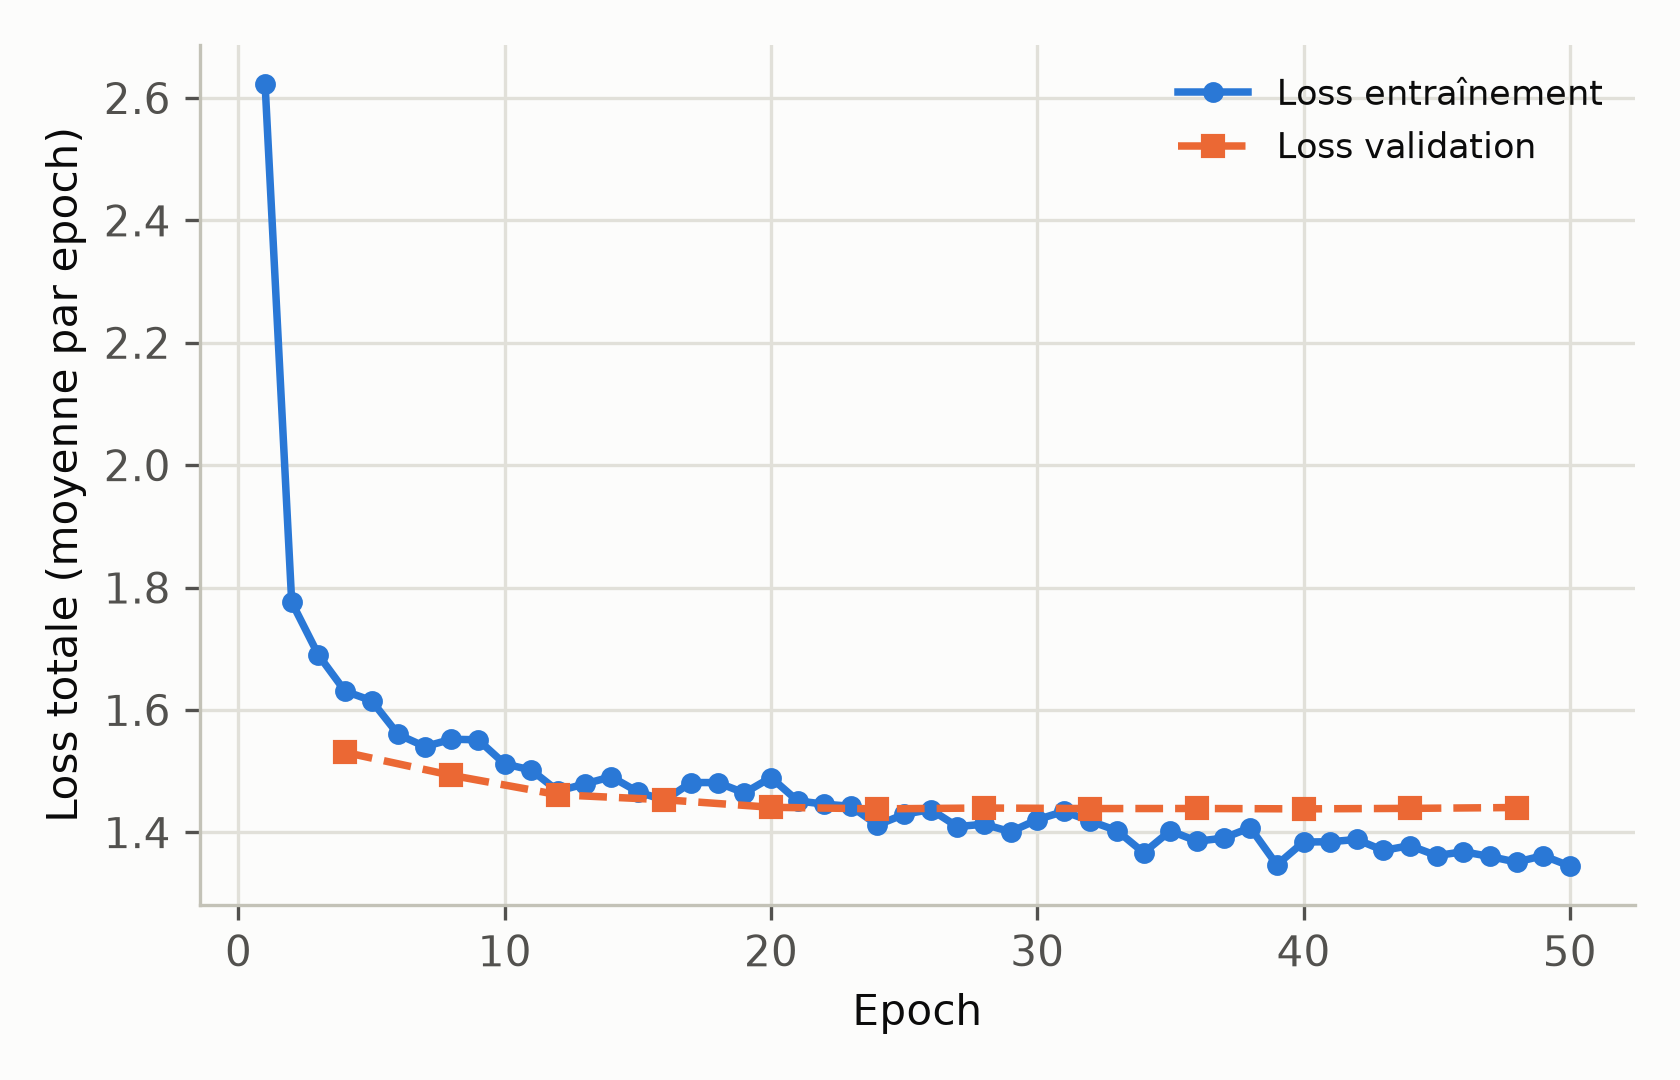
\includegraphics[width=0.7\textwidth]{figures/loss_curves_416px.png}
    \caption{Loss d'entraînement vs validation par epoch, génération 1
    (416px).}
    \end{figure}
    
    \subsubsection{Courbes de précision}
    
    \begin{figure}[!htbp]
    \centering
    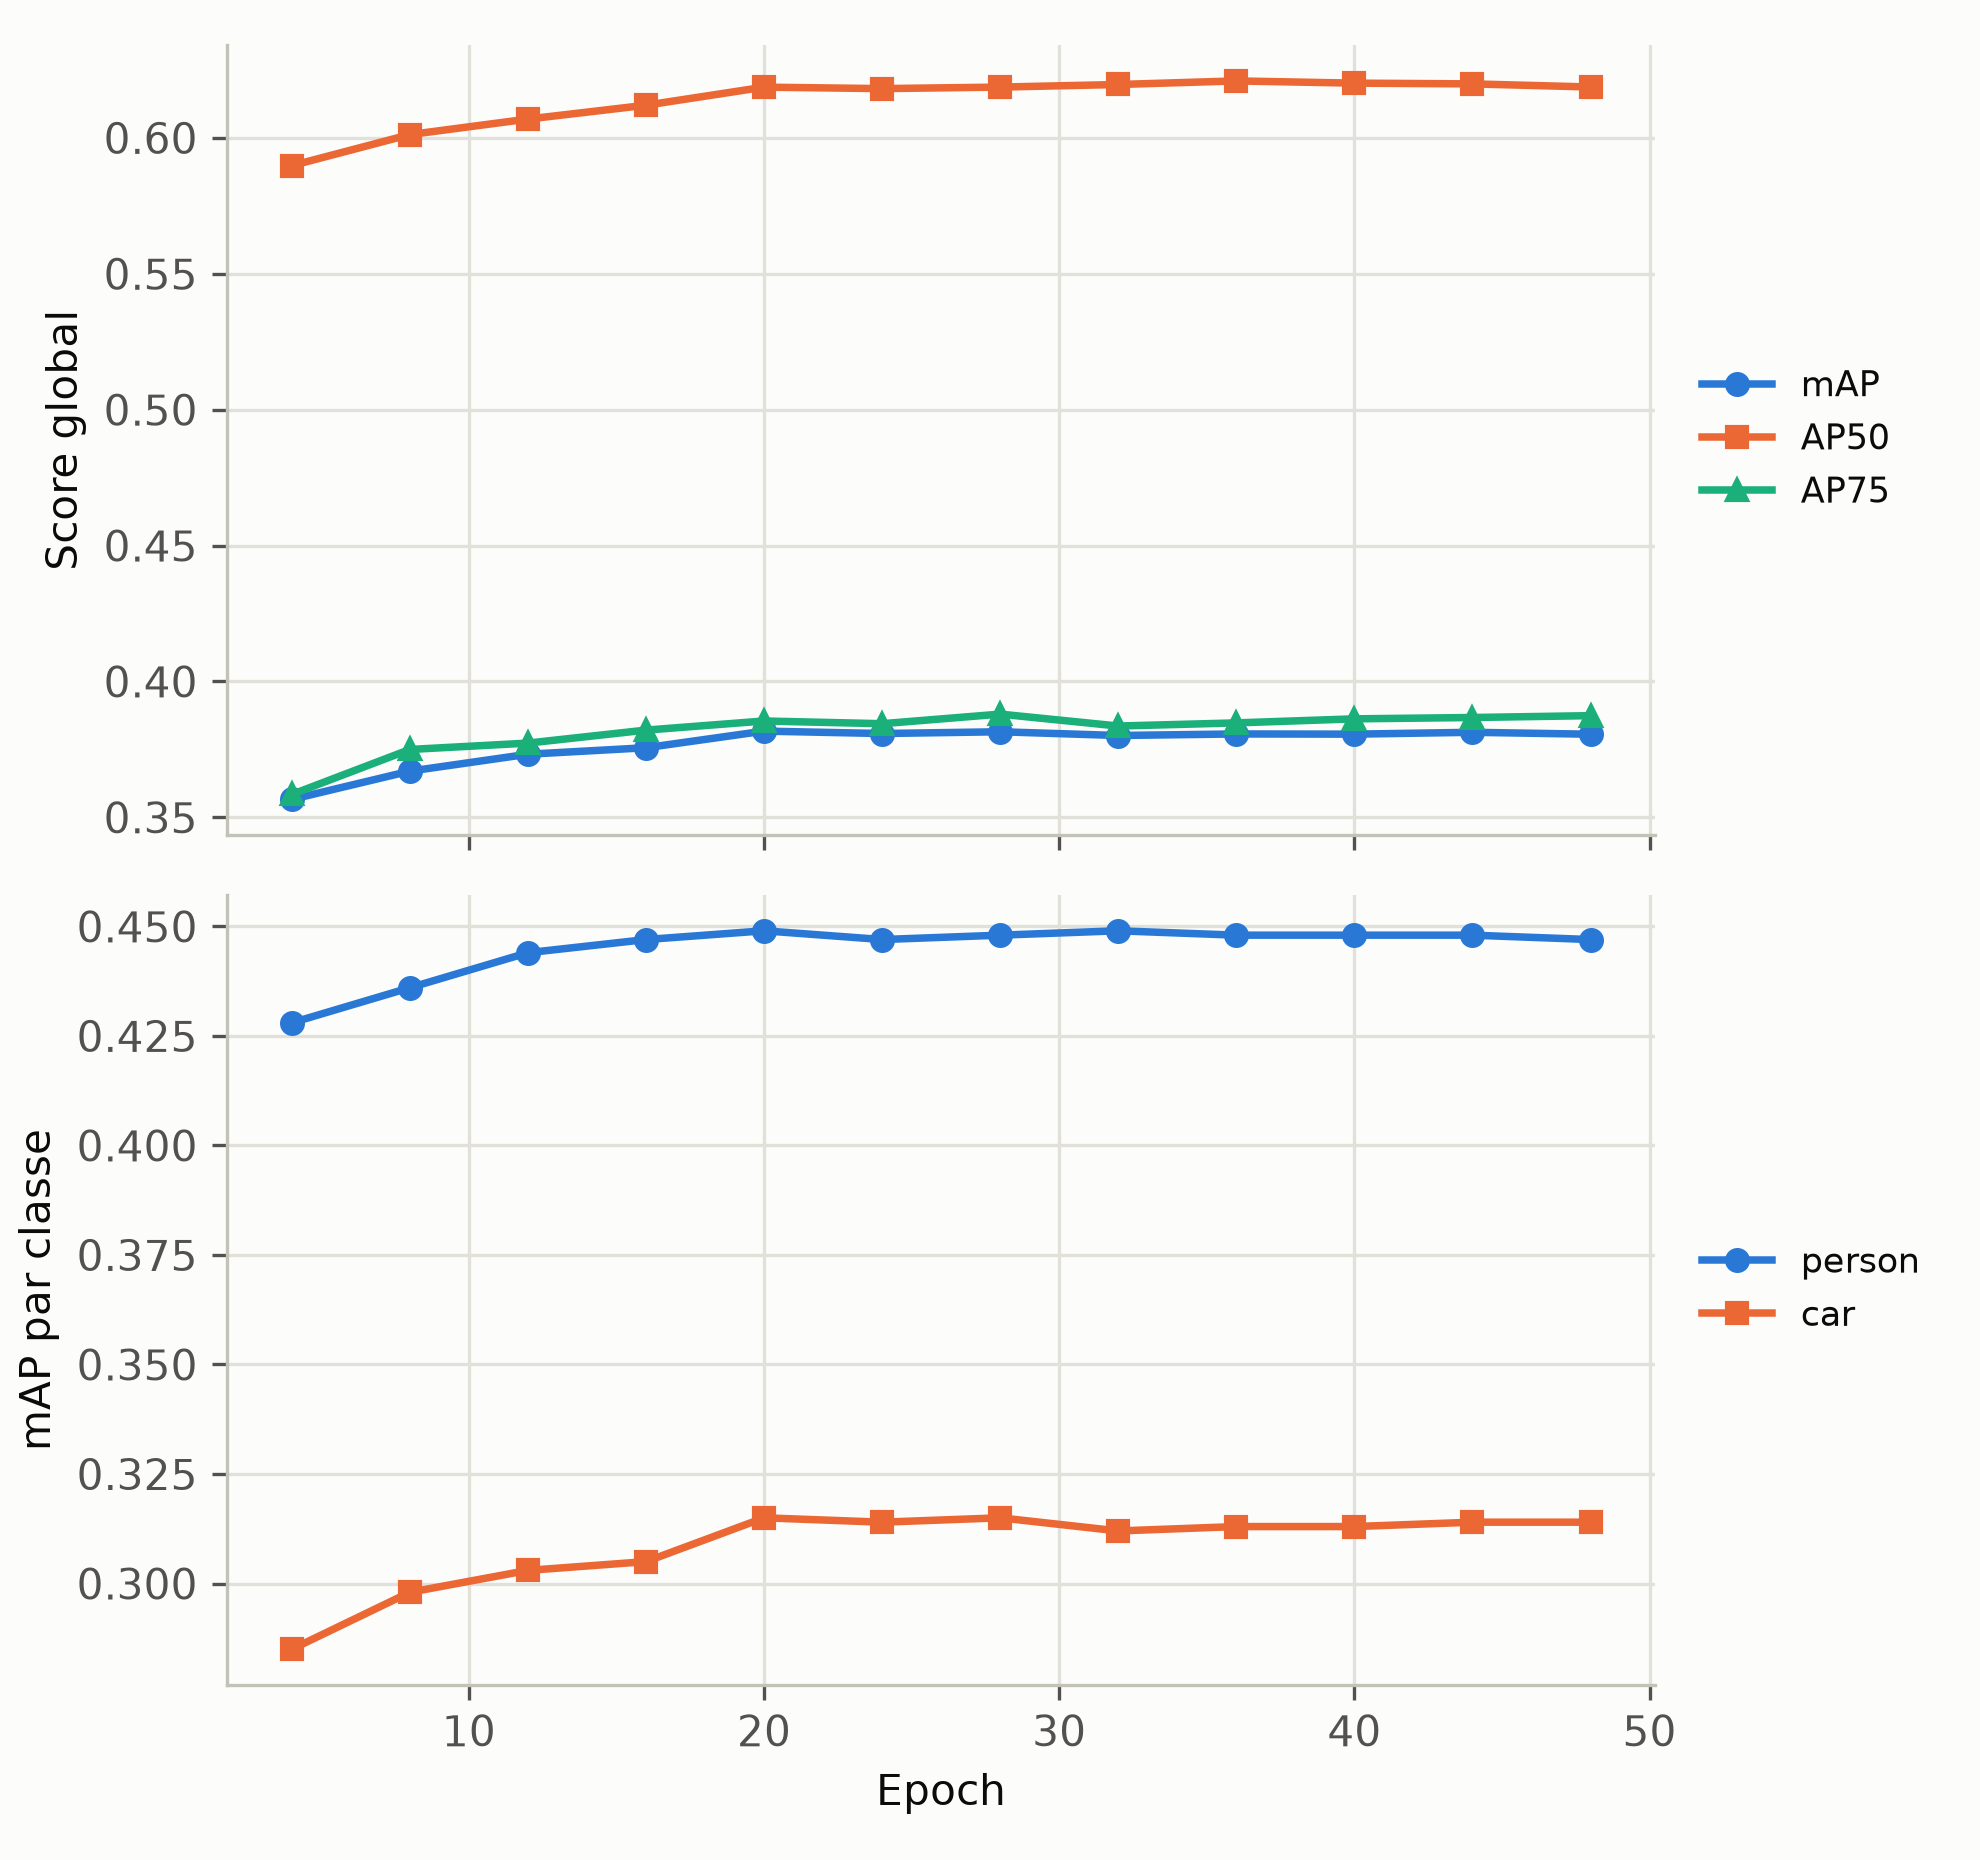
\includegraphics[width=0.75\textwidth]{figures/val_metrics_416px.png}
    \caption{Métriques de détection par epoch de validation, génération 1
    (416px) --- score global (mAP/AP50/AP75) et mAP par classe.}
    \end{figure}
    
    \subsubsection{Précision du meilleur modèle}
    
    Résultat sur \texttt{test.json} (fp32) :
    
    \begin{table}[!htbp]
    \centering
    \small
    \begin{adjustbox}{max width=\linewidth}
    \begin{tabular}{@{}lc@{}}
    \toprule
    \textbf{Métrique} & \textbf{416px fp32} \\
    \midrule
    mAP & \textbf{0,382} \\
    AP50 & 0,618 \\
    AP75 & 0,390 \\
    \texttt{AP\_small} & \textbf{0,175} \\
    \texttt{AP\_medium} & 0,540 \\
    \texttt{AP\_large} & 0,712 \\
    \bottomrule
    \end{tabular}
    \end{adjustbox}
    \end{table}
    
    On observe comme attendu un score nettement moins bon pour les petits objets (\texttt{AP\_small}) du à la faible résolution d'entrée.
    
    \subsection{Génération 2 --- passage à 512px}
    
    \subsubsection{Paramètres}
    
    Motivée par l'hypothèse de la section 2.4, cette génération bénéficie d'une résolution d'entrée de 512px, soit un gain de $151\%$ pixels.
    
    Les hyperparamètres ont été réajustés selon la même règle de mise à
    l'échelle proportionnelle batch/LR utilisée en génération 1 :
    
    \begin{table}[!htbp]
    \centering
    \small
    \begin{adjustbox}{max width=\linewidth}
    \begin{tabular}{@{}p{3.4cm}p{2.2cm}p{2.2cm}p{7.3cm}@{}}
    \toprule
    \textbf{Paramètre} & \textbf{416px (gén. 1)} & \textbf{512px (gén. 2)} & \textbf{Justification} \\
    \midrule
    \texttt{input\_size} & [416,416] & \textbf{[512,512]} & Teste directement l'hypothèse posée en section 2.4 sur les petits objets \\
    \texttt{batchsize\_per\_gpu} & 24 & \textbf{16} & Réduit proportionnellement ($24/1{,}51\approx16$) pour rester dans le même budget VRAM à $1{,}51\times$ plus de pixels/image \\
    \texttt{optimizer.lr} & 0,0001 & \textbf{0,00007} & Règle de mise à l'échelle linéaire batch/lr appliquée au nouveau batch \\
    \texttt{warmup.steps} & 200 & \textbf{300} & Prudence supplémentaire : le réseau doit reprendre le fine-tuning \emph{et} s'adapter à une résolution d'entrée différente \\
    \bottomrule
    \end{tabular}
    \end{adjustbox}
    \end{table}
    
    \texttt{total\_epochs} (50) et \texttt{val\_intervals} (4) restent
    \textbf{inchangés} par rapport à la génération 1 --- avec le jeu de
    données désormais constant entre les trois générations (section 3),
    la résolution d'entrée et les hyperparamètres qui en découlent
    mécaniquement (batch, LR, warmup) sont la \textbf{seule} chose qui
    diffère d'une génération à l'autre.
    
    \subsubsection{Courbes de loss}
    
    Le plateau s'est confirmé à l'\textbf{epoch 36} (\texttt{model\_best},
    mAP val=0,4165), avec une convergence stable en fin d'entraînement ---
    pas de recul marqué.
    
    \begin{figure}[!htbp]
    \centering
    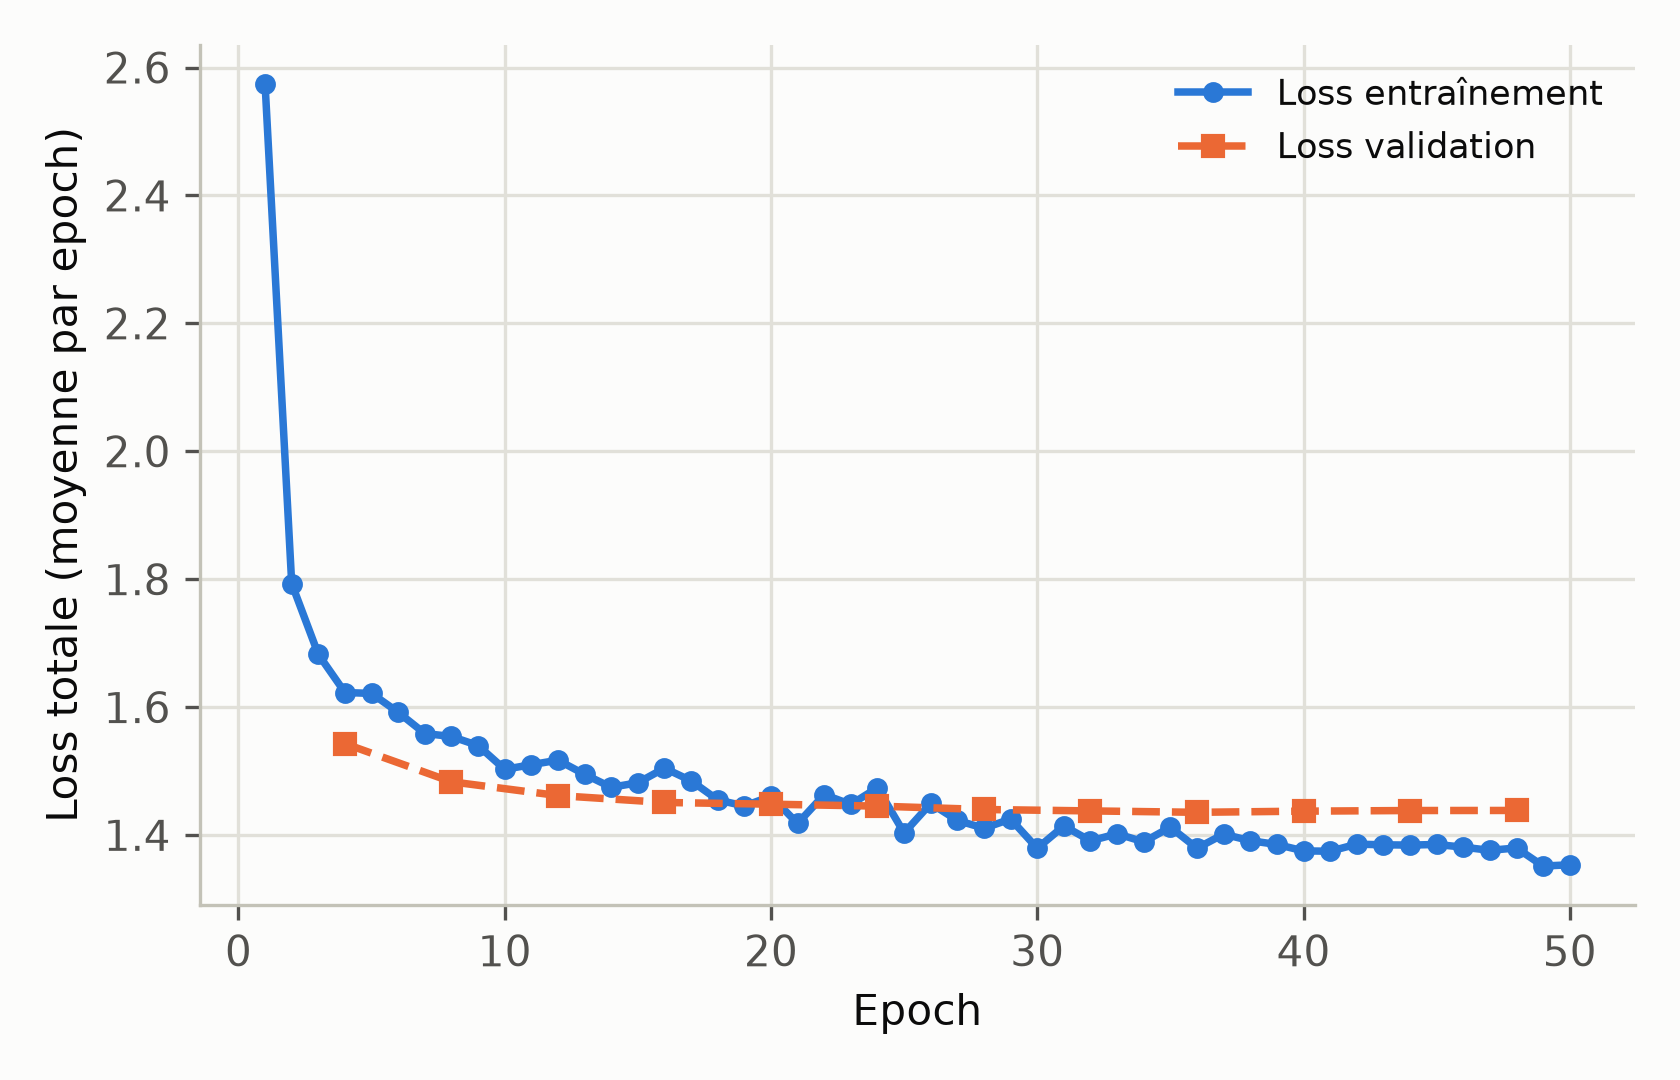
\includegraphics[width=0.7\textwidth]{figures/loss_curves_512px.png}
    \caption{Loss d'entraînement vs validation par epoch, génération 2
    (512px)}
    \end{figure}
    
    \subsubsection{Courbes de précision}
    
    \begin{figure}[!htbp]
    \centering
    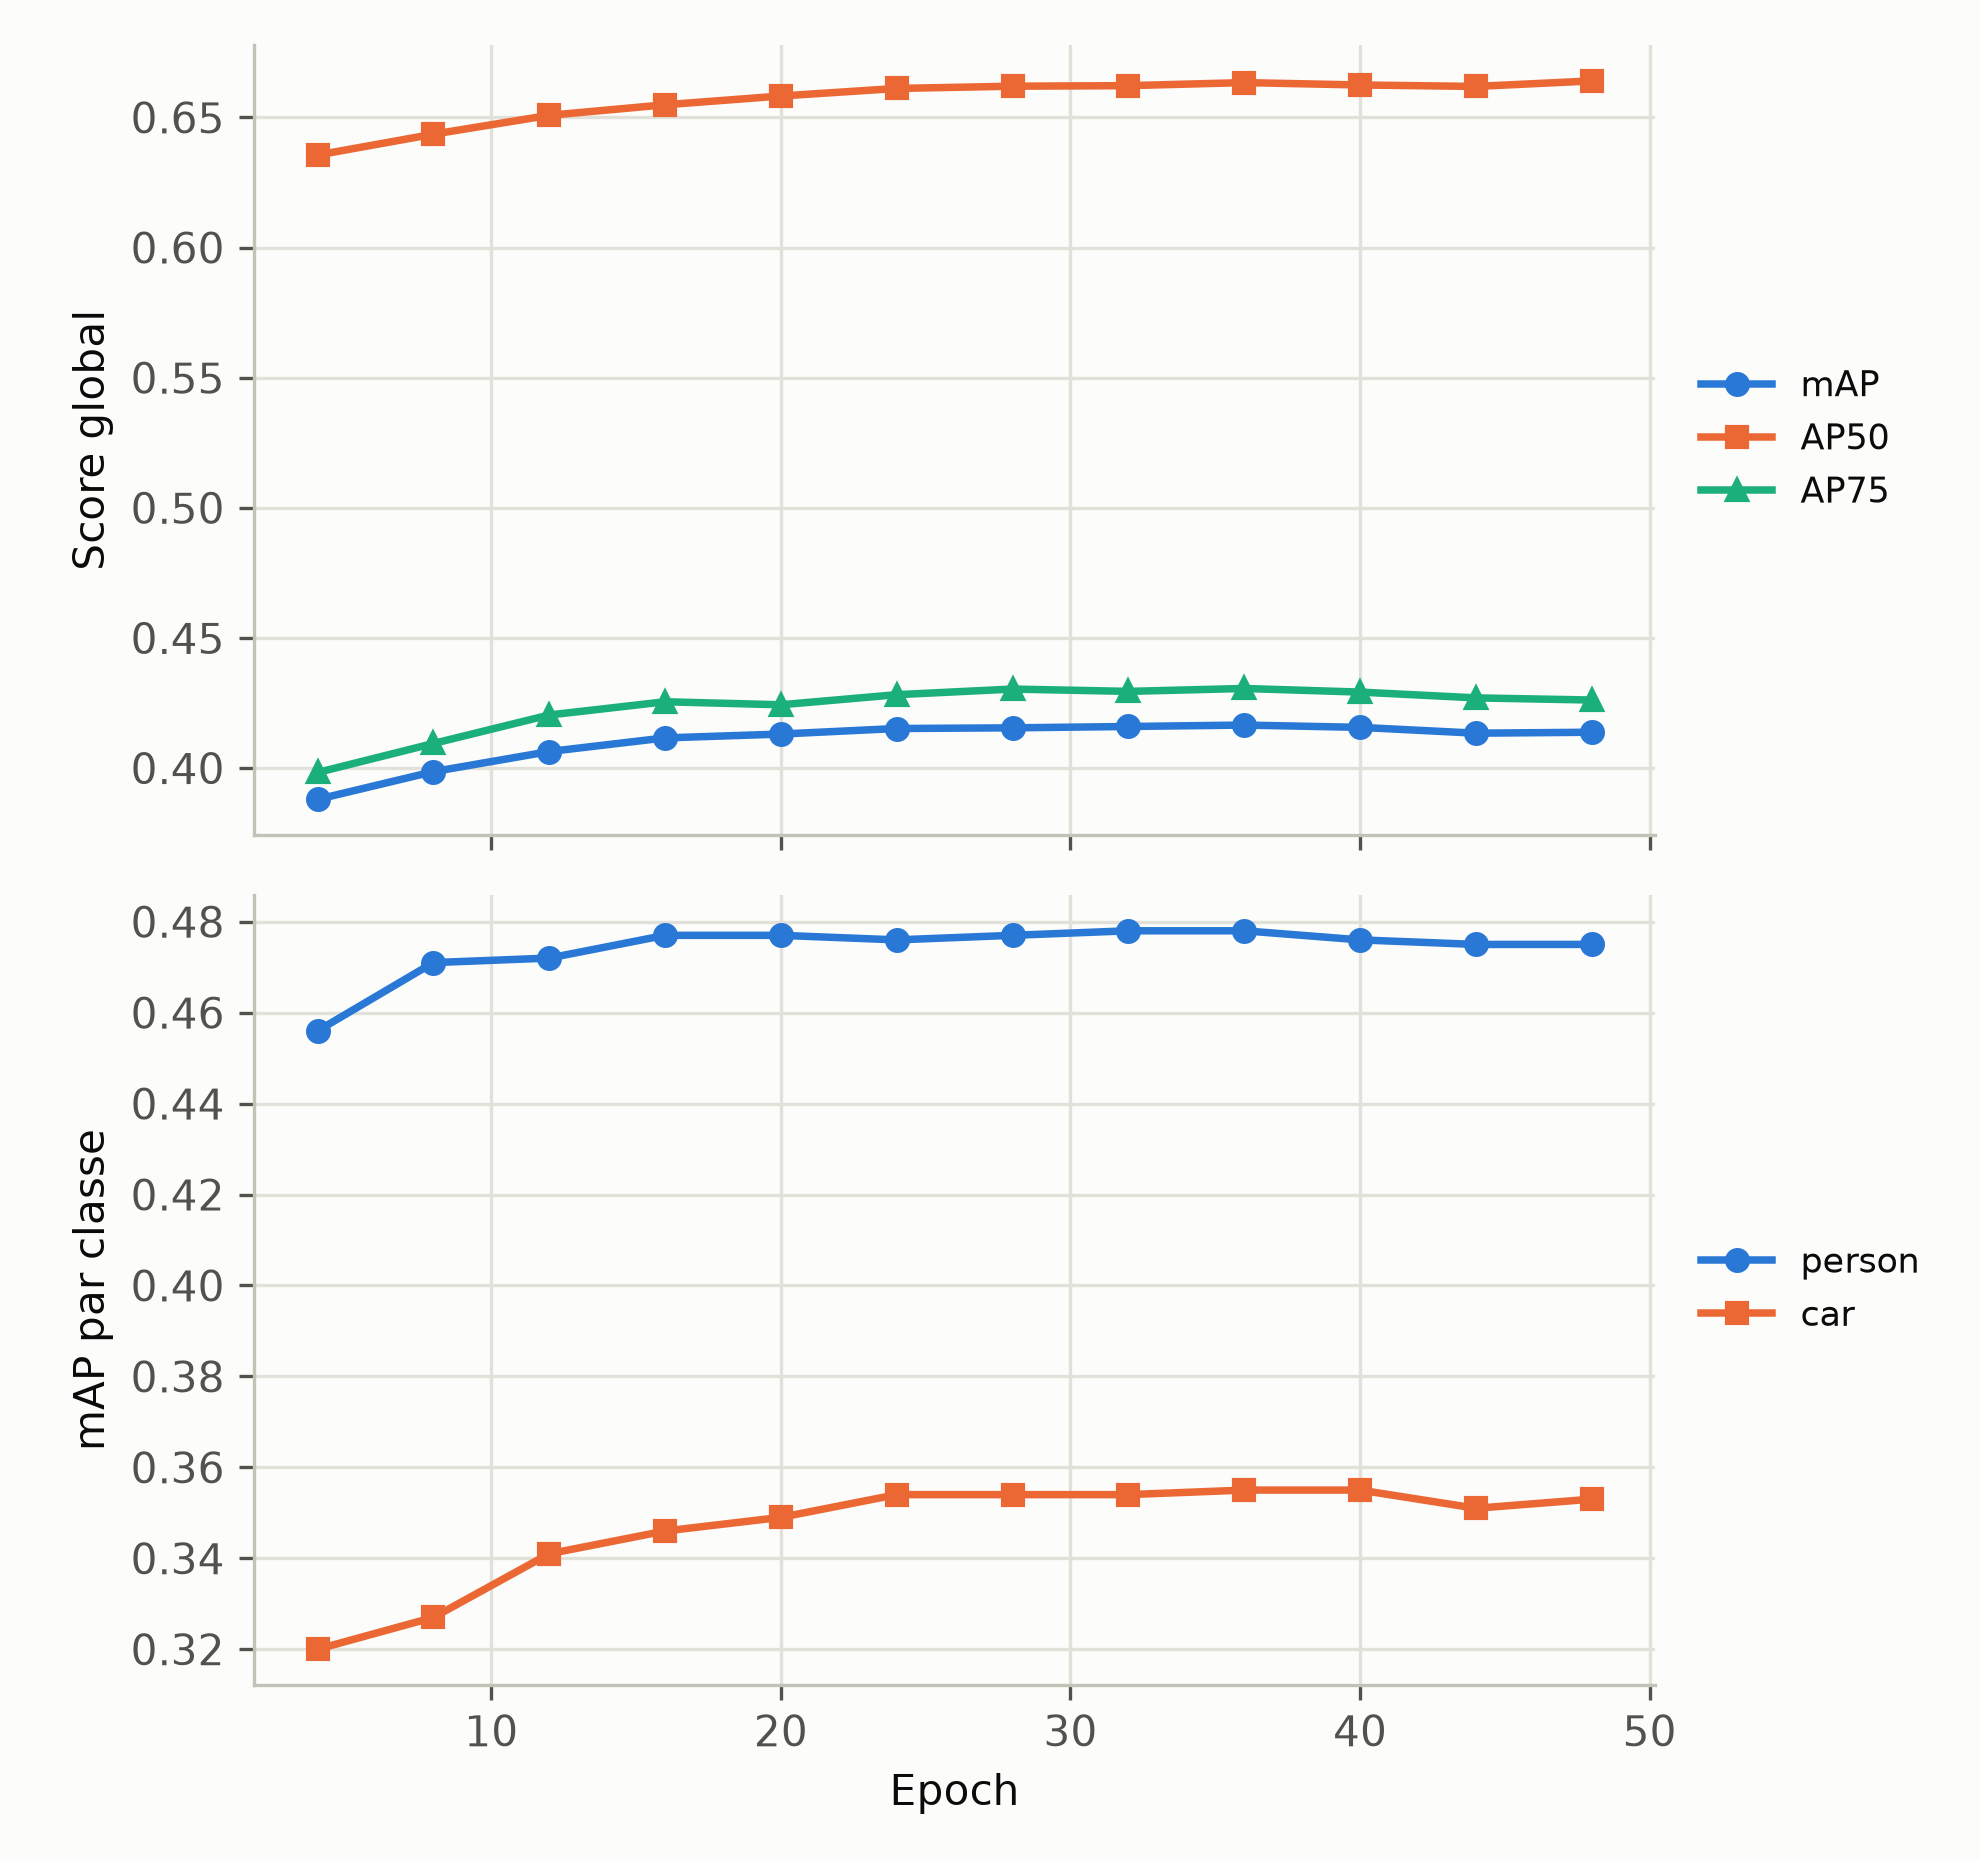
\includegraphics[width=0.75\textwidth]{figures/val_metrics_512px.png}
    \caption{Métriques de détection par epoch de validation, génération 2
    (512px) --- score global (mAP/AP50/AP75) et mAP par classe.}
    \end{figure}
    
    \subsubsection{Précision du meilleur modèle}
    
    Résultat sur \texttt{test.json} (fp32) :
    
    \begin{table}[!htbp]
    \centering
    \small
    \begin{adjustbox}{max width=\linewidth}
    \begin{tabular}{@{}lcc@{}}
    \toprule
    \textbf{Métrique} & \textbf{512px fp32} & \textbf{vs 416px} \\
    \midrule
    mAP & \textbf{0,421} & +10,2\% \\
    AP50 & 0,668 & +8,1\% \\
    AP75 & 0,438 & +12,3\% \\
    \texttt{AP\_small} & \textbf{0,228} & +30,3\% \\
    \texttt{AP\_medium} & 0,583 & +8,0\% \\
    \texttt{AP\_large} & 0,712 & +0,0\% \\
    \bottomrule
    \end{tabular}
    \end{adjustbox}
    \end{table}
    
    On observe le plus gros gain relatif sur la métrique \texttt{AP\_small}, augmentant de plus de  30\% ce qui semble confirmer l'hypothèse posée en
    section 2.4. Globalement cette résolution supérieur profite à toute les métrique à l'exception de \texttt{AP\_large} qui
    n'évolue pas du tout (0,712 dans les deux générations) --- cohérent
    avec l'idée que le gain de résolution profite spécifiquement aux
    petits objets, pas aux grands qui étaient déjà bien détectés.
    
    \subsection{Génération 3 --- recherche du plafond de résolution, 896px}
    
    \subsubsection{Paramètres}
    
    Le passage à 512px ayant confirmé l'hypothèse de départ
    (\texttt{AP\_small} en nette progression au fil de l'entraînement,
    section 4.2), la question naturelle était de savoir jusqu'où pousser
    la résolution avant que le compromis IPS ne devienne défavorable.
    Point méthodologique notable : la \textbf{latence d'un
    modèle ne dépend que de sa résolution et de son architecture, pas des
    poids entraînés}. Il est donc possible de mesurer le IPS à plusieurs
    résolutions candidates en export/quantifiant le modèle 512px
    \emph{déjà entraîné} à ces résolutions, \textbf{sans réentraîner} ---
    et donc sans engager des heures de calcul avant de savoir si la
    résolution visée est viable en pratique. Mesures effectuées
    sur le \textbf{candidat de déploiement} (ONNX INT8 QDQ \texttt{u8s8},
    CPU --- section 5.3), avec la même méthodologie que
    \texttt{benchmark.py} (section 6.1).
    
    \begin{table}[!htbp]
    \centering
    \small
    \begin{adjustbox}{max width=\linewidth}
    \begin{tabular}{@{}lcccc@{}}
    \toprule
    \textbf{Résolution} & \textbf{Latence médiane} & \textbf{IPS} & \textbf{P95} & \textbf{$\Delta$Mém} \\
    \midrule
    416 & 10,22 ms & 97,8 & 13,02 ms & 14,08 Mo \\
    512 & 13,67 ms & 73,2 & 16,85 ms & 20,04 Mo \\
    640 & 19,36 ms & 51,6 & 22,40 ms & 24,79 Mo \\
    768 & 26,73 ms & 37,4 & 30,13 ms & 44,29 Mo \\
    832 & 31,33 ms & 31,9 & 36,20 ms & 47,67 Mo \\
    \textbf{896} & \textbf{35,53 ms} & \textbf{28,1} & \textbf{41,38 ms} & \textbf{56,41 Mo} \\
    960 & 40,48 ms & \textbf{24,7} & 45,94 ms & 74,91 Mo \\
    1024 & 46,71 ms & 21,4 & 53,51 ms & 86,53 Mo \\
    \bottomrule
    \end{tabular}
    \end{adjustbox}
    \end{table}
    
    
    Le seuil de $\geq$25 IPS retenu (\S 1.1) est un \textbf{plancher} à
    respecter, pas un objectif à dépasser largement --- le même
    type de critère que la taille maximale en section 2.3. Sur les huit résolutions mesurées ci-dessus, \textbf{896px est
    le dernier palier qui respecte encore ce plancher} (28,1 IPS,
    $\sim$12\% de marge) : \textbf{960px repasse sous le seuil} (24,7
    IPS, en inférence pure seule --- avant même le reste du pipeline réel :
    décodage boîtes/NMS, tracker, affichage, qui ne fait qu'ajouter de la
    latence), et 1024px est nettement en dessous.
    
    \textbf{896px est donc retenu directement} comme résolution de la
    génération 3 --- un saut de résolution substantiel vs 512px
    ($\times$3,06 en pixels), au prix d'un
    coût de calcul en conséquence ($\sim$31h de calcul actif, réparties en
    deux segments séparés par une pause manuelle de 48 heures après l'epoch
    35 --- section 4.3.2).
    
    Les hyperparamètres ont de nouveau été réajustés proportionnellement :
    
    \begin{table}[!htbp]
    \centering
    \small
    \begin{adjustbox}{max width=\linewidth}
    \begin{tabular}{@{}p{3.4cm}p{2.2cm}p{2.2cm}p{6.8cm}@{}}
    \toprule
    \textbf{Paramètre} & \textbf{512px (gén. 2)} & \textbf{896px (gén. 3)} & \textbf{Justification} \\
    \midrule
    \texttt{input\_size} & [512,512] & \textbf{[896,896]} & Résolution retenue ci-dessus \\
    \texttt{batchsize\_per\_gpu} & 16 & \textbf{6} & $16/(896/512)^2\approx5{,}2$, arrondi à 6 \\
    \texttt{optimizer.lr} & 0,00007 & \textbf{0,00002625} & $\times(6/16)$, même règle de mise à l'échelle \\
    \texttt{warmup.steps} & 300 & \textbf{450} & Prudence supplémentaire, saut de résolution plus grand qu'en génération 2 \\
    \bottomrule
    \end{tabular}
    \end{adjustbox}
    \end{table}
    
    \subsubsection{Courbes de loss}
    
    Le plateau final se confirme à l'\textbf{epoch
    30} (\texttt{model\_best}, mAP val=0,4813).
    
    \begin{figure}[!htbp]
    \centering
    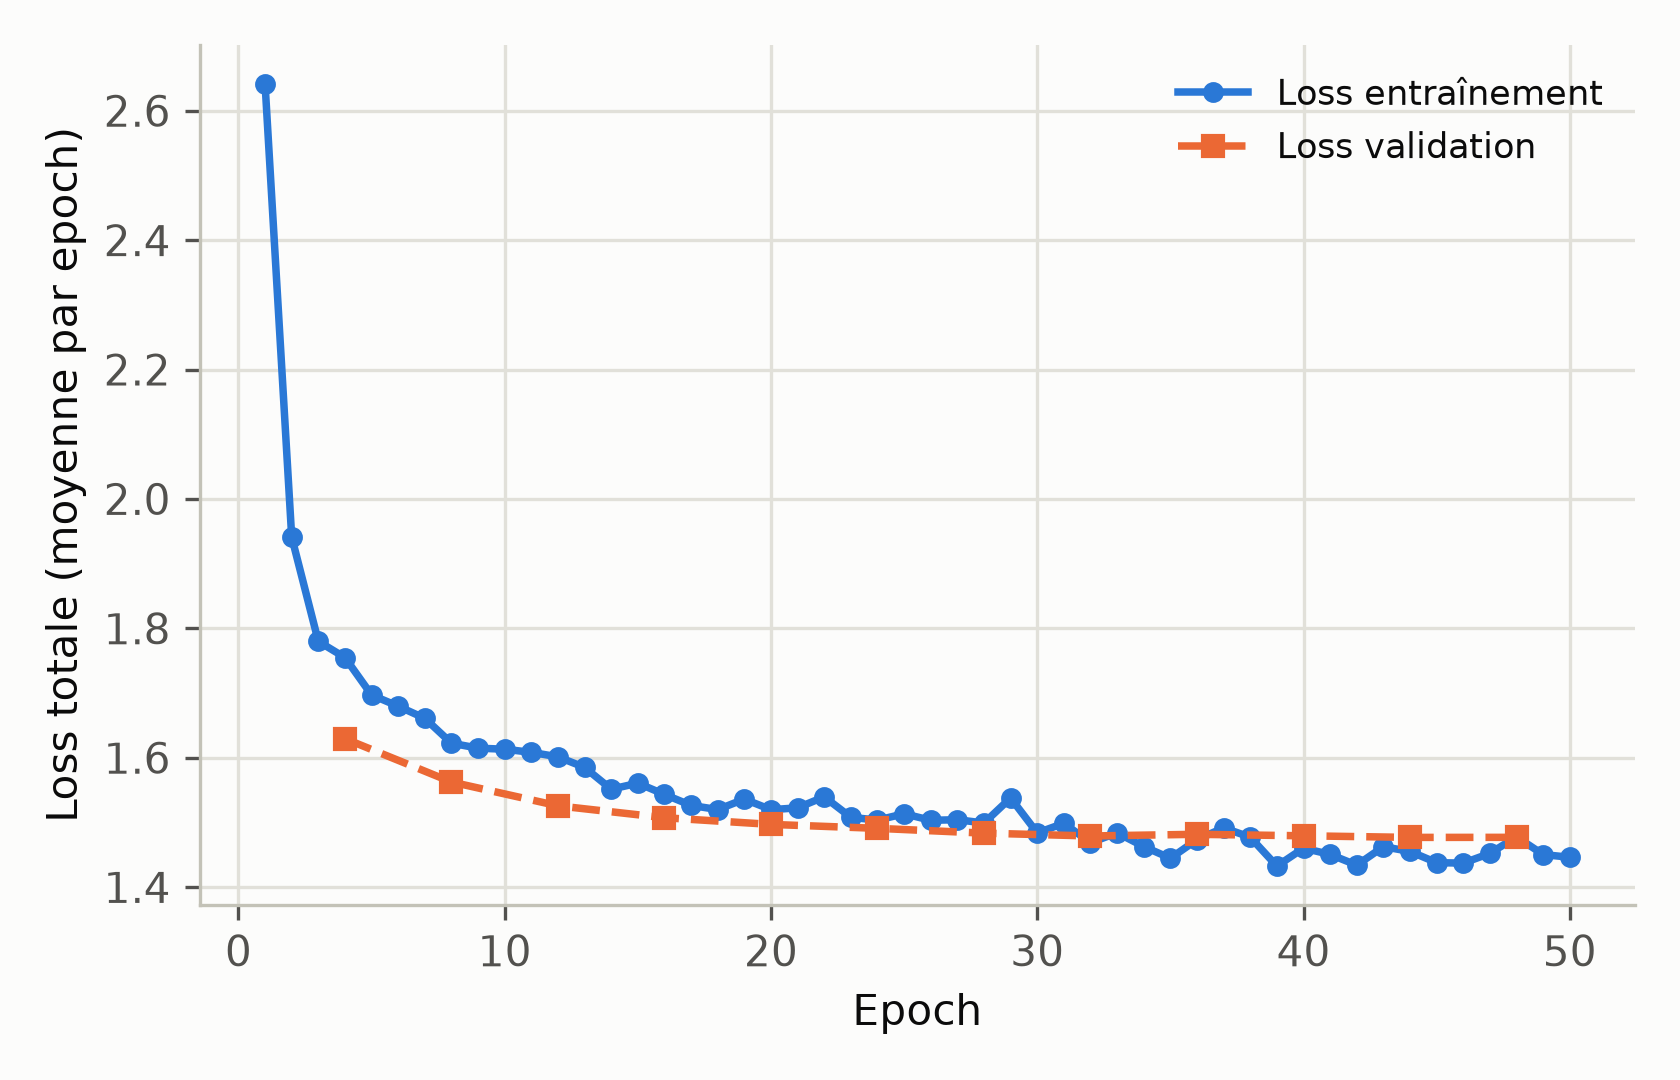
\includegraphics[width=0.7\textwidth]{figures/loss_curves_896px.png}
    \caption{Loss d'entraînement vs validation par epoch, génération 3
    (896px). Convergence sans décrochage, aucun signe de sur-apprentissage
    sur cette métrique ; les deux courbes restent proches d'un bout à
    l'autre, comme pour les autres générations (section 4.1).}
    \end{figure}
    
    \subsubsection{Courbes de précision}
    
    \begin{figure}[!htbp]
    \centering
    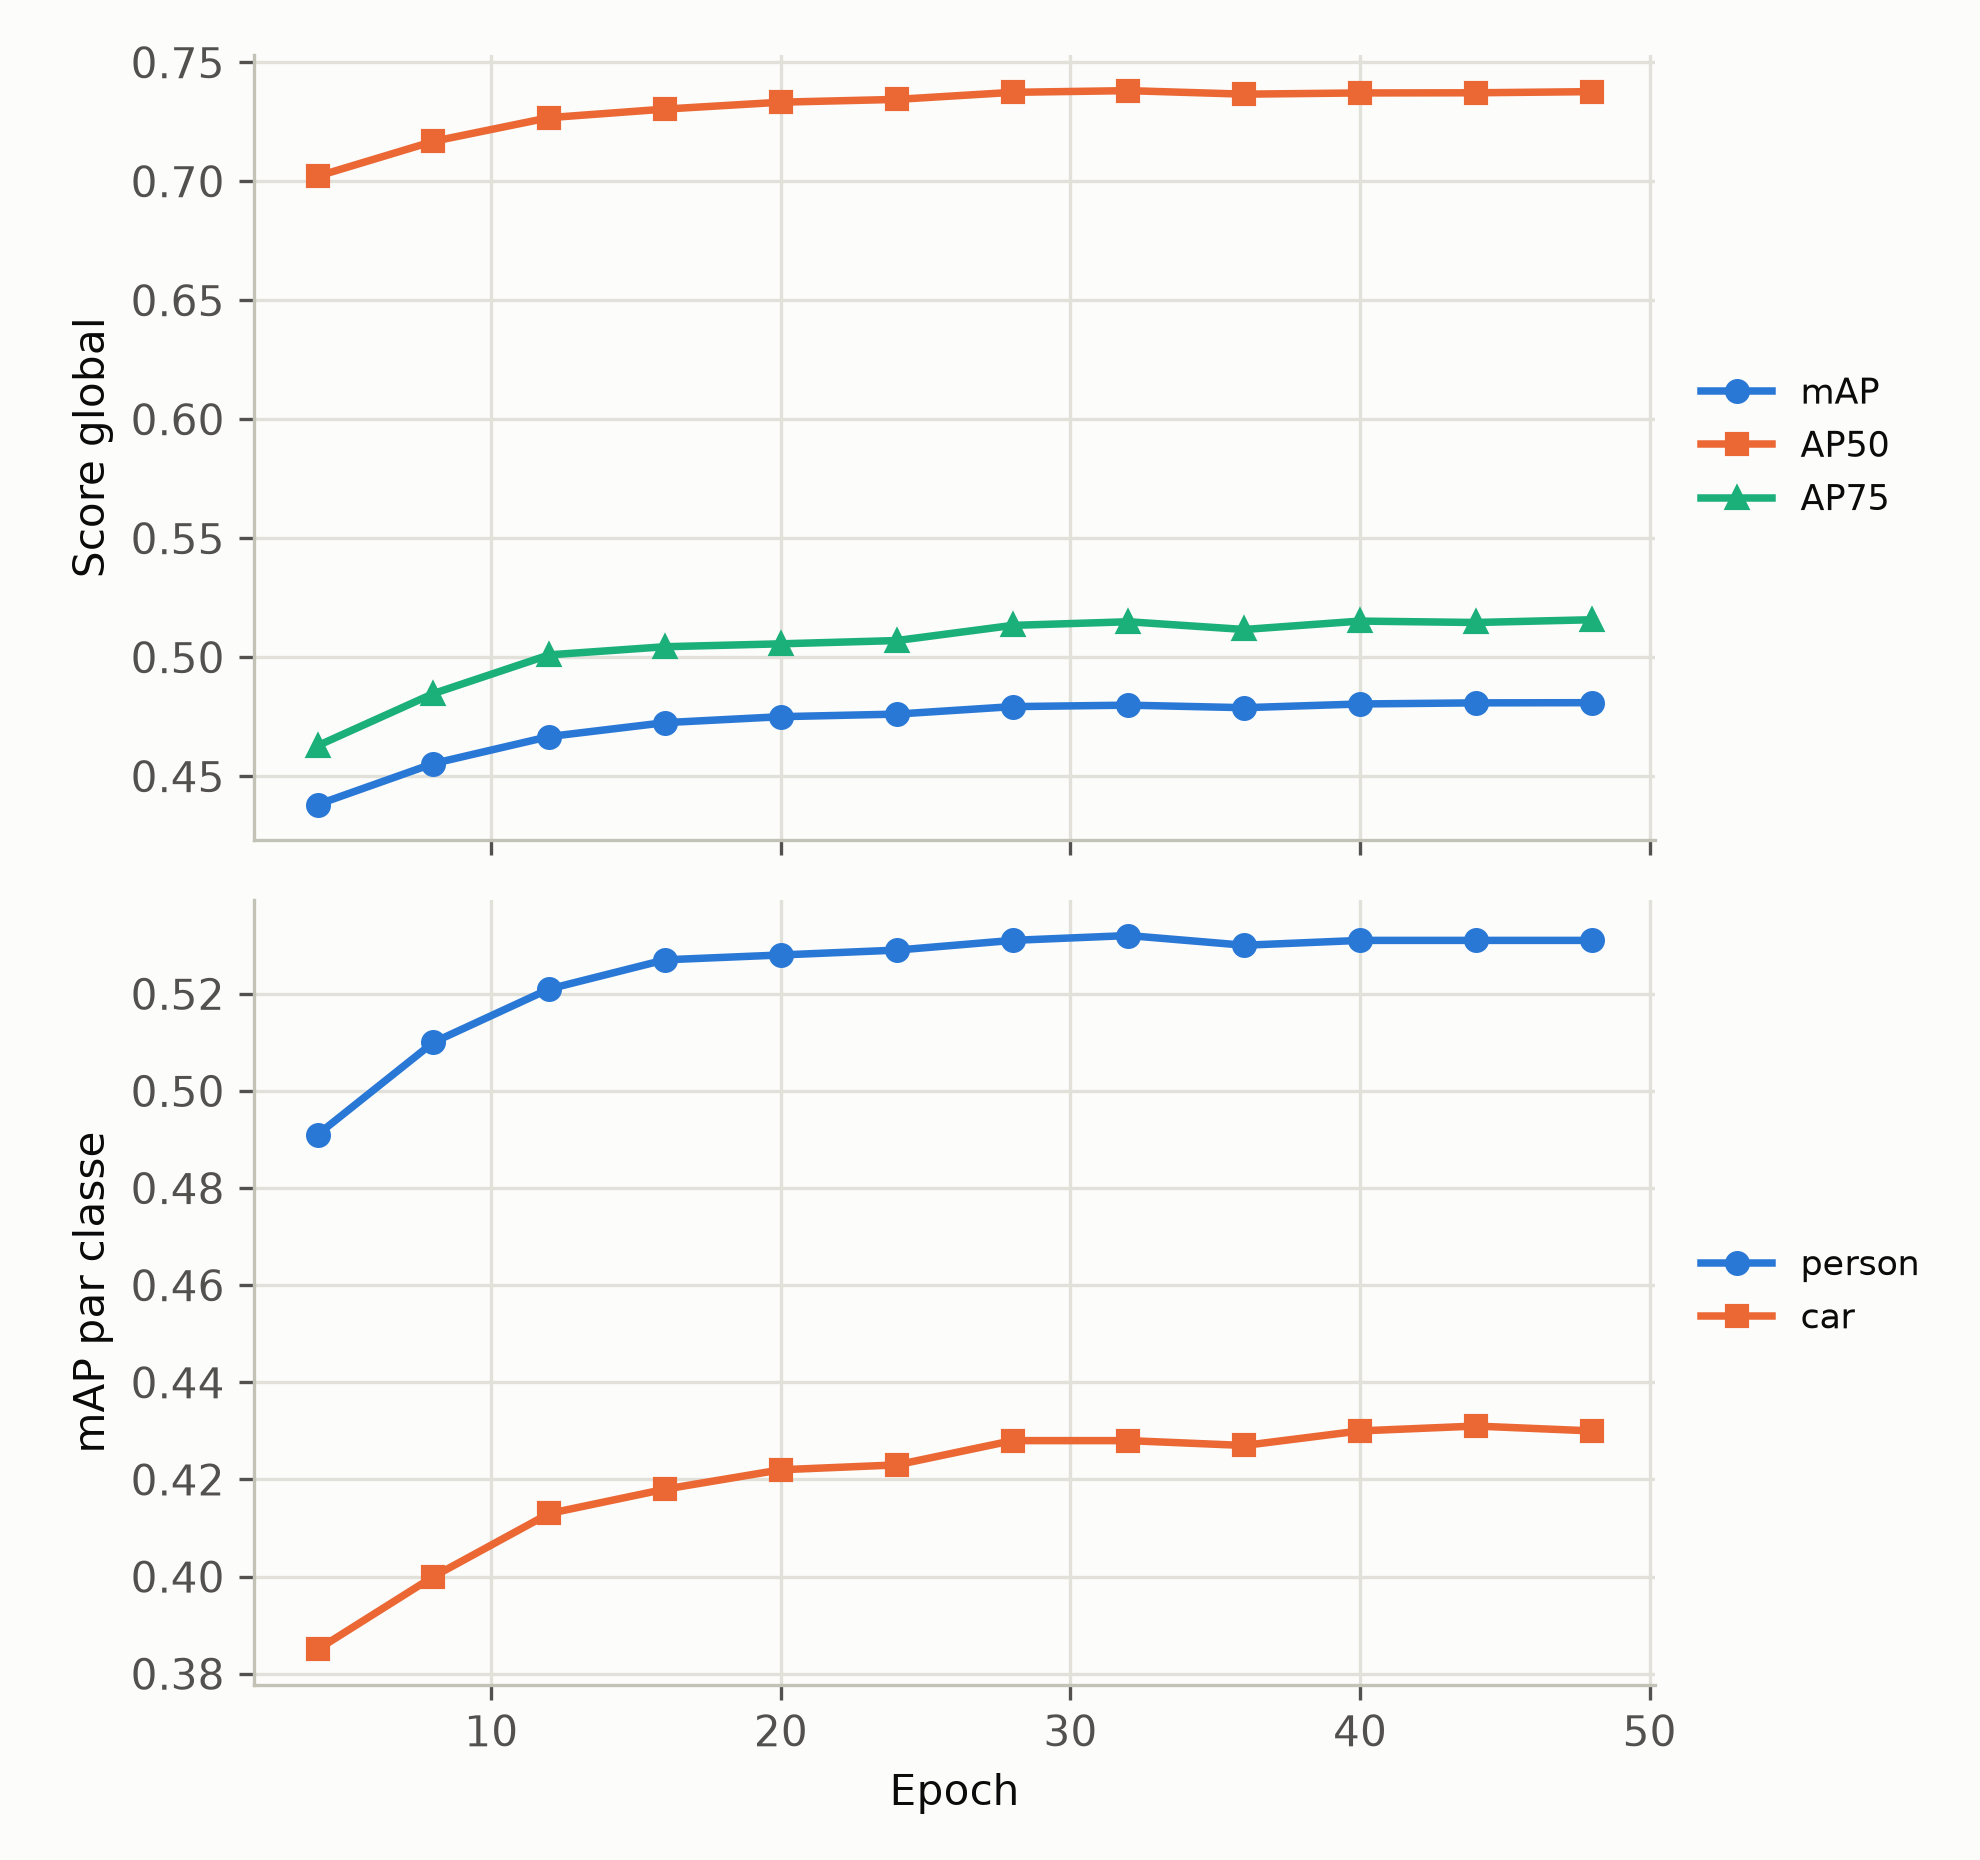
\includegraphics[width=0.75\textwidth]{figures/val_metrics_896px.png}
    \caption{Métriques de détection par epoch de validation, génération 3
    (896px) --- score global (mAP/AP50/AP75) et mAP par classe. Progression
    monotone jusqu'au plateau ($\sim$epoch 30), sans recul notable ensuite.}
    \end{figure}
    
    \subsubsection{Précision du meilleur modèle}
    
    Résultat final sur \texttt{test.json} (fp32) :
    
    \begin{table}[!htbp]
    \centering
    \small
    \begin{adjustbox}{max width=\linewidth}
    \begin{tabular}{@{}lccc@{}}
    \toprule
    \textbf{Métrique} & \textbf{896px fp32} & \textbf{vs 512px} & \textbf{vs 416px} \\
    \midrule
    mAP & \textbf{0,485} & +15,2\% & +27,0\% \\
    AP50 & 0,739 & +10,6\% & +19,6\% \\
    AP75 & 0,509 & +16,2\% & +30,5\% \\
    \texttt{AP\_small} & \textbf{0,335} & +46,9\% & \textbf{+91,4\%} \\
    \texttt{AP\_medium} & 0,629 & +7,9\% & +16,5\% \\
    \texttt{AP\_large} & 0,684 & -3,9\% & -3,9\% \\
    \bottomrule
    \end{tabular}
    \end{adjustbox}
    \end{table}
    
    Seule \texttt{AP\_large} recule (-3,9\%) --- cohérent avec une
    hypothèse plausible (la résolution redistribue une partie de la
    capacité du modèle vers les petits objets, un peu au détriment des
    grands) mais non vérifiée plus finement ici, sans que ça remette en
    cause le gain global. Sur l'ensemble de la progression 416px$\to$896px,
    \texttt{AP\_small} cumule un gain de \textbf{+91,4\%} --- de loin la
    métrique la plus transformée par la hausse de résolution, cohérent de
    bout en bout avec l'hypothèse posée dès la section 2.4.
    
    \subsection{Bilan de progression}
    
    Comparaison des meilleurs modèles (\texttt{model\_best}) des trois
    générations, fp32, sur \texttt{test.json} --- mêmes 6 métriques que
    les tableaux de précision de chaque génération (sections 4.1--4.3) :
    
    \begin{table}[!htbp]
    \centering
    \small
    \begin{adjustbox}{max width=\linewidth}
    \begin{tabular}{@{}lccc@{}}
    \toprule
    \textbf{Métrique} & \textbf{416px (gén. 1)} & \textbf{512px (gén. 2)} & \textbf{896px (gén. 3)} \\
    \midrule
    mAP & 0,382 & 0,421 & \textbf{0,485} \\
    AP50 & 0,618 & 0,668 & \textbf{0,739} \\
    AP75 & 0,390 & 0,438 & \textbf{0,509} \\
    \texttt{AP\_small} & 0,175 & 0,228 & \textbf{0,335} \\
    \texttt{AP\_medium} & 0,540 & 0,583 & \textbf{0,629} \\
    \texttt{AP\_large} & \textbf{0,712} & \textbf{0,712} & 0,684 \\
    \bottomrule
    \end{tabular}
    \end{adjustbox}
    \end{table}
    
    Ratio \texttt{person:car} (mAP, \texttt{model\_best}) des trois
    générations, à comparer au ratio brut des annotations du jeu de
    données (1,47, section 3.2) :
    
    \begin{table}[!htbp]
    \centering
    \small
    \begin{adjustbox}{max width=\linewidth}
    \begin{tabular}{@{}lccc@{}}
    \toprule
    & \textbf{416px (gén. 1)} & \textbf{512px (gén. 2)} & \textbf{896px (gén. 3)} \\
    \midrule
    person (mAP) & 44,8\% & 47,8\% & \textbf{53,2\%} \\
    car (mAP) & 31,2\% & 35,7\% & \textbf{43,1\%} \\
    ratio person:car & 1,44 & 1,34 & \textbf{1,23} \\
    \bottomrule
    \end{tabular}
    \end{adjustbox}
    \end{table}
    
    Le ratio mesuré sur les modèles (1,44 puis
    1,34 puis 1,23) reste à chaque génération \textbf{inférieur} au ratio
    brut des annotations du jeu de données (1,47), et se resserre de façon
    monotone sur les 3 générations --- l'entraînement ne se contente pas
    d'hériter du déséquilibre des données, il le compense partiellement,
    et ce gain s'accentue avec la résolution plutôt que de stagner. Le
    déséquilibre n'est cependant jamais éliminé (le ratio reste $>$1 à
    chaque génération).
    
    
    \section{Quantification INT8 --- toolchain maison}
    
    \subsection{Pipeline général}
    
    La quantification post-entraînement (PTQ) est développée entièrement en
    interne, sans dépendre d'un outil clé-en-main : \textbf{export ONNX
    $\to$ validation numérique $\to$ calibration $\to$ quantification PTQ
    $\to$ validation taille/précision}. Chaque étape est un script Python
    autonome (\texttt{export\_onnx.py}, \texttt{validate\_onnx.py},
    \texttt{quantize.py}, \texttt{evaluate\_int8.py}), détaillés dans les
    sous-sections suivantes.
    
    \subsection{Export et validation}
    
    Le graphe est exporté avec \texttt{torch.onnx.export}, puis
    simplifié avec \texttt{onnxsim} et validé structurellement avec
    \texttt{onnx.checker}. La liste des opérateurs présents dans le graphe
    final est inspectée explicitement : \textbf{aucun opérateur de NMS
    n'apparaît} --- confirmation directe, sur le graphe réellement exporté
    et non plus seulement sur la documentation de l'architecture, du
    critère « graphe exporté propre » posé en section 2.2.
    
    La fidélité numérique de l'export est vérifiée sur 3 images de test
    réelles, en comparant la sortie brute PyTorch (fp32) à la sortie ONNX
    sur le même tenseur d'entrée : écart maximal mesuré \mbox{1,1--1,7
    $\times 10^{-5}$} (tolérances standard
    \texttt{rtol=1e-3}, \texttt{atol=1e-5}) --- l'export ne dégrade pas la
    précision du modèle.
    
    \subsection{Choix du format d'export et du type d'activation}
    
    Avant même de choisir une méthode de calibration, deux paramètres de
    \texttt{quantize\_static} restent à trancher : le format d'export et
    le type des activations. Toutes les mesures de cette section sont
    faites sur le \textbf{modèle final 896px}, pour rester directement
    comparables au modèle effectivement déployé plutôt qu'à des
    résolutions intermédiaires depuis retirées, avec une calibration
    \texttt{MinMax} tenue constante pour isoler ces deux seules variables.
    
    \subsubsection{Type des activations : \texttt{u8s8} contre \texttt{s8s8}}
    
    Deux combinaisons possibles pour le signe des poids/activations
    quantifiés :
    
    \begin{itemize}[leftmargin=1.5em]
      \item \textbf{\texttt{s8s8}} --- poids et activations tous deux en
        int8 signé --- le choix qui semblait le plus simple au départ.
      \item \textbf{\texttt{u8s8}} --- activations en uint8 non signé,
        poids en int8 signé.
    \end{itemize}
    
    Mesuré au banc (\texttt{benchmark.py}, warmup 15, 150 mesures, format
    \texttt{QDQ} tenu constant pour isoler cette seule variable) :
    
    \begin{table}[!htbp]
    \centering
    \small
    \begin{adjustbox}{max width=\linewidth}
    \begin{tabular}{@{}lcc@{}}
    \toprule
    \texttt{QDQ} & \texttt{s8s8} & \texttt{u8s8} \\
    \midrule
    Latence médiane & 90,4 ms & \textbf{31,4 ms} \\
    IPS & 11,1 & \textbf{31,8} \\
    \bottomrule
    \end{tabular}
    \end{adjustbox}
    \end{table}
    
    Le format \texttt{s8s8} rend l'INT8 nettement plus lent que le format
    \texttt{u8s8}. Après étude de la documentation, il s'avère que sur CPU
    x86-64 avec extensions AVX2/AVX512, \texttt{onnxruntime} exécute la
    combinaison
    \texttt{u8}$\times$\texttt{s8} via l'instruction SIMD dédiée
    \texttt{VPMADDUBSW} (remplacée par l'instruction native VNNI sur les
    CPU qui la supportent, sans le risque de saturation propre à
    \texttt{VPMADDUBSW} sur AVX2/AVX512 seul) --- un chemin de calcul
    rapide qui n'a pas d'équivalent pour \texttt{s8}$\times$\texttt{s8},
    d'où le repli sur un chemin générique bien plus lent\footnote{ONNX
    Runtime, \emph{Quantize ONNX Models} ---
    \url{https://onnxruntime.ai/docs/performance/model-optimizations/quantization.html},
    section « Data type selection ».}.
    
    \subsubsection{Format d'export : \texttt{QDQ} contre \texttt{QOperator}}
    
    Ici aussi, deux choix candidats retenus, avec \texttt{u8s8} désormais
    fixé :
    
    \begin{itemize}[leftmargin=1.5em]
      \item \textbf{\texttt{QDQ}} --- paires \texttt{QuantizeLinear}/\texttt{DequantizeLinear}
        explicites dans le graphe, portable : n'importe quel runtime peut
        les fusionner en noyaux int8 à sa façon.
      \item \textbf{\texttt{QOperator}} --- opérateurs quantifiés dédiés
        directement dans le graphe, plus compact mais moins portable.
    \end{itemize}
    
    Taille du fichier (\texttt{u8s8} dans les deux cas) :
    
    \begin{table}[!htbp]
    \centering
    \small
    \begin{adjustbox}{max width=\linewidth}
    \begin{tabular}{@{}lc@{}}
    \toprule
    \textbf{Format} & \textbf{Taille} \\
    \midrule
    \texttt{QOperator} & \textbf{2,80 Mo} \\
    \texttt{QDQ} & 3,12 Mo \\
    \bottomrule
    \end{tabular}
    \end{adjustbox}
    \end{table}
    
    \texttt{QOperator} produit un fichier $\sim$10\% plus léger. Mais la
    contrainte du projet est un \textbf{plafond} de 5 Mo (section 1.1),
    déjà largement respecté par les deux formats --- ce n'est donc pas la
    taille qui doit trancher ici, contrairement à la vitesse :
    
    \begin{table}[!htbp]
    \centering
    \small
    \begin{adjustbox}{max width=\linewidth}
    \begin{tabular}{@{}lcc@{}}
    \toprule
    \texttt{u8s8} & \texttt{QDQ} & \texttt{QOperator} \\
    \midrule
    Latence médiane & \textbf{31,4 ms} & 39,6 ms \\
    IPS & \textbf{31,8} & 25,2 \\
    \bottomrule
    \end{tabular}
    \end{adjustbox}
    \end{table}
    
    \texttt{QOperator} reste plus lent que \texttt{QDQ} même une fois
    \texttt{u8s8} (à 896px, la combinaison la plus défavorable des
    quatre, \texttt{QOperator}+\texttt{s8s8}, atteint même 383,3 ms/2,6 IPS,
    loin derrière les trois autres). Ayant
    déjà le budget de taille largement respecté, autant exploiter la
    marge de vitesse disponible plutôt que de gagner un peu de poids déjà
    non contraignant.
    
    \subsection{Calibration PTQ --- premier choix et sa limite}
    
    Le premier réglage considéré fut la calibration
    \texttt{MinMax} sur 200 images, avec le format \texttt{QDQ}+\texttt{u8s8}
    retenu en section 5.3 --- le plus simple pour une première approche,
    sans hyperparamètre à régler. Résultat sur \texttt{test.json}
    (896px) :
    
    \begin{table}[!htbp]
    \centering
    \small
    \begin{adjustbox}{max width=\linewidth}
    \begin{tabular}{@{}lcccccc@{}}
    \toprule
    & \textbf{mAP} & \textbf{AP50} & \textbf{AP75} & \textbf{\texttt{AP\_small}} & \textbf{\texttt{AP\_medium}} & \textbf{\texttt{AP\_large}} \\
    \midrule
    fp32 & 0,485 & 0,739 & 0,509 & 0,335 & 0,629 & 0,684 \\
    INT8 (\texttt{MinMax}) & 0,4377 & 0,6878 & 0,4579 & 0,2897 & 0,5892 & 0,6066 \\
    \midrule
    \textbf{Perte vs fp32} & \textbf{-9,7\%} & -6,9\% & -10,0\% & \textbf{-13,5\%} & -6,3\% & -11,3\% \\
    \bottomrule
    \end{tabular}
    \end{adjustbox}
    \end{table}
    
    Perte substantielle et inégale selon les métriques --- particulièrement
    marquée sur \texttt{AP\_small} (-13,5\%), cohérent avec l'idée que les
    petits objets, déjà les plus difficiles, sont aussi les plus sensibles
    à la perte de précision numérique de la quantification.
    
    Cette première approche s'avère sensible aux valeurs
    aberrantes de calibration : \texttt{MinMax} fixe l'échelle de
    quantification sur le min/max \emph{observé} des activations, une
    méthode connue pour ce défaut
    
    \begin{table}[!htbp]
    \centering
    \small
    \begin{adjustbox}{max width=\linewidth}
    \begin{tabular}{@{}lc@{}}
    \toprule
    \textbf{N images de calibration} & \textbf{mAP} \\
    \midrule
    100 & \textbf{0,4428} \\
    200 (retenu) & 0,4377 \\
    500 & 0,4308 \\
    1000 & 0,4299 \\
    \bottomrule
    \end{tabular}
    \end{adjustbox}
    \end{table}
    
    Le mAP se \textbf{dégrade} de façon monotone quand le nombre d'images
    de calibration augmente --- résultat contre-intuitif, mais cohérent
    avec le fonctionnement de \texttt{MinMax} : plus le nombre d'images
    grandit, plus la probabilité de rencontrer une activation extrême
    augmente, étirant artificiellement la plage de quantification au
    détriment du cas normal majoritaire. Cette
    sensibilité aux valeurs aberrantes motive directement la recherche
    d'une méthode de calibration plus robuste.
    
    \subsection{Vers une meilleure calibration}
    
    Deux méthodes de calibration à histogramme, \texttt{Percentile} et
    \texttt{Entropy}, sont conceptuellement conçues pour être plus
    robustes aux valeurs aberrantes que le min/max brut : plutôt que de
    fixer l'échelle sur les valeurs extrêmes observées, elles s'appuient
    sur la distribution complète des activations. Testées dans les mêmes
    conditions (\texttt{QDQ}+\texttt{u8s8}, N=200, modèle 896px) :
    
    \begin{table}[!htbp]
    \centering
    \footnotesize
    \begin{adjustbox}{max width=\linewidth}
    \begin{tabular}{@{}lcccccc@{}}
    \toprule
    & \textbf{mAP} & \textbf{AP50} & \textbf{AP75} & \textbf{\texttt{AP\_small}} & \textbf{\texttt{AP\_medium}} & \textbf{\texttt{AP\_large}} \\
    \midrule
    fp32 & 0,485 & 0,739 & 0,509 & 0,335 & 0,629 & 0,684 \\
    \midrule
    \texttt{MinMax} & 0,4377 (-9,7\%) & 0,6878 (-6,9\%) & 0,4579 (-10,0\%) & 0,2897 (-13,5\%) & 0,5892 (-6,3\%) & 0,6066 (-11,3\%) \\
    \texttt{Entropy} & 0,4549 (-6,2\%) & 0,7063 (-4,4\%) & 0,4774 (-6,2\%) & 0,2989 (-10,8\%) & 0,6070 (-3,5\%) & 0,6305 (-7,8\%) \\
    \textbf{\texttt{Percentile}} & \textbf{0,4623 (-4,7\%)} & \textbf{0,7165 (-3,0\%)} & \textbf{0,4877 (-4,2\%)} & \textbf{0,3099 (-7,5\%)} & \textbf{0,6109 (-2,9\%)} & \textbf{0,6522 (-4,7\%)} \\
    \bottomrule
    \end{tabular}
    \end{adjustbox}
    \end{table}
    
    Au-delà de gagner sur les valeurs absolues, \texttt{Percentile} est
    aussi la méthode qui \textbf{perd le moins face au fp32} sur
    \textbf{chacune} des 6 métriques,
    +5,6\% de mAP relatif vs \texttt{MinMax}.
    \texttt{Entropy} bat légèrement \texttt{MinMax} mais reste nettement
    derrière \texttt{Percentile}. Le choix retenu serat donc d'utiliser \texttt{Percentile} comme méthode de calibration.
    
    \subsection{Résultat de quantification (modèle final, 896px)}
    
    Décomposition du fichier QDQ final par type de tenseur :
    
    \begin{table}[!htbp]
    \centering
    \begin{adjustbox}{max width=\linewidth}
    \begin{tabular}{@{}lrrr@{}}
    \toprule
    \textbf{Dtype} & \textbf{Tenseurs} & \textbf{Poids} & \textbf{\%} \\
    \midrule
    \texttt{int8}  & 220 & 2,4208 Mo & 89,93\% \\
    \texttt{float32} (scales)        & 445 & 0,1357 Mo &  5,04\% \\
    \texttt{int32} (biais quantifiés) & 220 & 0,1348 Mo &  5,01\% \\
    \texttt{int64} (constantes graphe) & 14 & 0,0003 Mo &  0,01\% \\
    \texttt{uint8} (zero-points activation) & 224 & 0,0002 Mo &  0,01\% \\
    \midrule
    \textbf{Total} & \textbf{1123} & \textbf{2,6918 Mo} & \textbf{100\%} \\
    \bottomrule
    \end{tabular}
    \end{adjustbox}
    \caption{Décomposition exhaustive des 1123 tenseurs statiques du modèle final (896px, QDQ, u8s8) par type de donnée brut.}
    \label{tab:dtype-breakdown}
    \end{table}
    
    Sans surprise, les poids de convolution (\texttt{int8}) dominent
    totalement le poids du modèle (89,9\%) --- c'est le seul poste que la
    quantification per-channel réduit réellement d'un facteur 4 par
    rapport au fp32 d'origine. Les biais, systématiquement quantifiés en
    \texttt{int32} par ONNX Runtime (jamais en dessous de 4 octets/valeur,
    quel que soit le format d'export choisi), et les métadonnées de
    quantification (\emph{scales} en \texttt{float32}, zero-points en
    \texttt{int8}/\texttt{int32}/\texttt{uint8}) ne représentent ensemble
    que 10,1\% du poids total. Les 1123 tenseurs recensés ici ne couvrent
    que les données brutes stockées dans le graphe : le fichier
    \texttt{.onnx} final pèse 3,121 Mo sur disque, soit 0,429 Mo (13,7\%)
    de plus --- un \emph{overhead} de structure (noms des nœuds, attributs
    des opérateurs, topologie du graphe) plutôt que des poids au sens
    propre.
    \\\\
    Comparaison fp32 / INT8 final sur les 6 métriques de détection
    (\texttt{test.json}) :
    
    \begin{table}[!htbp]
    \centering
    \small
    \begin{adjustbox}{max width=\linewidth}
    \begin{tabular}{@{}lcccccc@{}}
    \toprule
    & \textbf{mAP} & \textbf{AP50} & \textbf{AP75} & \textbf{\texttt{AP\_small}} & \textbf{\texttt{AP\_medium}} & \textbf{\texttt{AP\_large}} \\
    \midrule
    fp32 & 0,485 & 0,739 & 0,509 & 0,335 & 0,629 & 0,684 \\
    INT8 final & \textbf{0,462} & 0,717 & 0,488 & 0,310 & 0,611 & 0,652 \\
    \midrule
    \textbf{Perte vs fp32} & \textbf{-4,7\%} & -3,0\% & -4,1\% & -7,5\% & -2,9\% & -4,7\% \\
    \bottomrule
    \end{tabular}
    \end{adjustbox}
    \end{table}
    
    \textbf{Précision finale, résolution 896px} : mAP fp32 = 0,485 $\to$
    mAP INT8 = 0,462, soit une perte de \textbf{-4,7\%} --- un peu plus
    marquée qu'à 768px (-3,2\%, mesuré en cours de projet avec la même
    toolchain), cohérent avec une résolution d'entrée plus fine qui laisse
    davantage de place à l'erreur de quantification sur les détails fins,
    sans remettre en cause le choix de la toolchain elle-même.
    
    \textbf{Contrainte de taille ($\leq$ 5 Mo) respectée avec marge
    confortable} : 3,12 Mo, soit 38\% de marge.
    
    
    \section{Performance et compromis précision/vitesse}
    
    \subsection{Méthodologie de benchmark}
    
    Le banc de mesure (\texttt{benchmark.py}) applique le même
    protocole à chaque candidat : 15 itérations de \emph{warmup} (écartées
    des statistiques, pour ne pas mesurer les effets de cache/JIT à
    froid), puis 150 mesures. Sont rapportés la moyenne, la médiane,
    l'écart-type, le minimum, le maximum, le P95 et le IPS dérivé de la
    médiane. La mémoire résidente (RSS) est échantillonnée toutes les 10
    itérations, avec une précaution méthodologique délibérée : la RSS de
    référence (\texttt{baseline}) est mesurée \textbf{avant la construction
    du modèle ou de la session} d'inférence, pas seulement avant la boucle
    de mesure --- pour capturer le coût réel de chargement du modèle en
    mémoire, pas seulement la croissance pendant les appels répétés.
    Contrairement à \texttt{quantize.py} et \texttt{evaluate\_int8.py}
    (section 5), \texttt{benchmark.py} ne limite \textbf{pas} l'affinité
    CPU du processus : la mesure de performance doit refléter les
    conditions réelles d'exécution, non un environnement artificiellement
    contraint.
    
    \subsection{Résultats comparés}
    
    Comparatif au modèle final (896px), fp32 GPU/CPU et candidat de
    déploiement INT8 :
    
    \begin{table}[!htbp]
    \centering
    \small
    \begin{adjustbox}{max width=\linewidth}
    \begin{tabular}{@{}lcc@{}}
    \toprule
    \textbf{Candidat} & \textbf{Latence médiane} & \textbf{IPS} \\
    \midrule
    PyTorch fp32 GPU & 9,39 ms & 106,5 \\
    PyTorch fp32 CPU & 168,15 ms & 5,9 \\
    \textbf{ONNX INT8 QDQ CPU (\texttt{u8s8}, retenu)} & \textbf{37,14 ms} & \textbf{26,9} \\
    \bottomrule
    \end{tabular}
    \end{adjustbox}
    \end{table}
    
    
    Le \textbf{GPU l'emporte nettement} ici (9,39 ms contre 37,14 ms) ---
    cohérent avec un modèle de cette taille, où le calcul brut pèse
    davantage face au coût fixe du transfert CPU$\leftrightarrow$GPU. Le
    candidat retenu reste néanmoins le CPU INT8 : la cible visée par ce
    projet est l'inférence embarquée (section 1.1), pas un poste équipé
    d'un GPU dédié.
    
    IPS et mémoire du candidat de déploiement selon la résolution
    d'entrée (avec même toolchian de quantification) --- ici la résolution a un vrai coût, contrairement à la
    taille du fichier (section 5.6) :
    
    \begin{table}[!htbp]
    \centering
    \small
    \begin{adjustbox}{max width=\linewidth}
    \begin{tabular}{@{}lccc@{}}
    \toprule
    & \textbf{416px} & \textbf{512px} & \textbf{896px} \\
    \midrule
    Latence médiane (CPU, INT8) & 9,99 ms & 16,50 ms & \textbf{37,14 ms} \\
    IPS (CPU, INT8) & 100,1 & 60,6 & \textbf{26,9} \\
    $\Delta$Mém (RSS) & 12,1 Mo & 21,3 Mo & \textbf{56,5 Mo} \\
    \bottomrule
    \end{tabular}
    \end{adjustbox}
    \end{table}
    
    La perte de IPS entre 416px et 896px est substantielle (100,1
    $\to$ 26,9, -73\%) et strictement monotone avec la résolution ---
    directement en tension avec le gain de précision, lui aussi monotone
    et substantiel (mAP fp32 +27,0\% entre les deux mêmes points, section
    4.4). La mémoire RSS augmente elle aussi avec la résolution du modèle, car les tenseurs d'activations à mémoriser temporairement sur une passe sont plus grand.
    
    \subsection{Arbitrage final}
    
    \textbf{896px est retenu} comme résolution de déploiement : meilleure
    précision des trois générations (mAP INT8 = 0,462, section 5.6), et
    IPS mesuré (26,9) qui \textbf{reste au-dessus} du seuil de $\geq$25 IPS
    retenu (\S 1.1) --- avec une marge plus resserrée qu'anticipé sur la
    mesure architecture-only de la section 4.3 (28,1 IPS), cohérent avec la
    variance déjà observée entre sessions de mesure distinctes sur ce poste
    de développement (section 7).

    Les deux figures ci-dessous montrent ce que ces chiffres donnent sur
    des images du jeu de test (modèle INT8 déployé, seuil de score 0,5) :
    détections du modèle en orange, vérité terrain COCO en vert.

    \begin{figure}[!htbp]
    \centering
    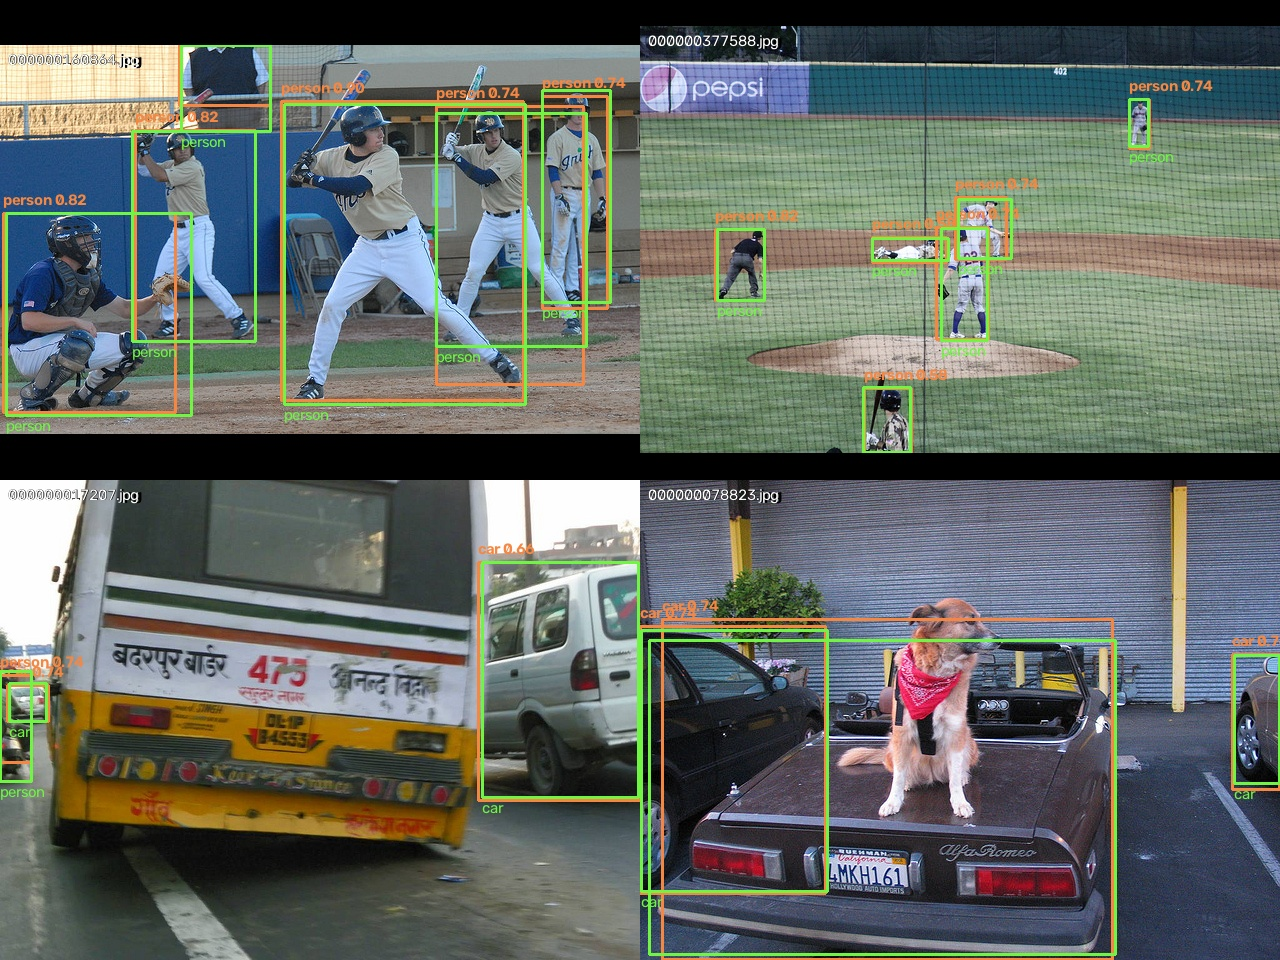
\includegraphics[width=0.9\textwidth]{figures/predictions_reussites.jpg}
    \caption{Cas réussis : personnes et voitures de taille moyenne à
    grande, toutes détectées sans faux positif. Le bus (en bas à gauche)
    n'appartient pas aux classes apprises et n'est pas détecté, comme
    attendu.}
    \end{figure}

    \begin{figure}[!htbp]
    \centering
    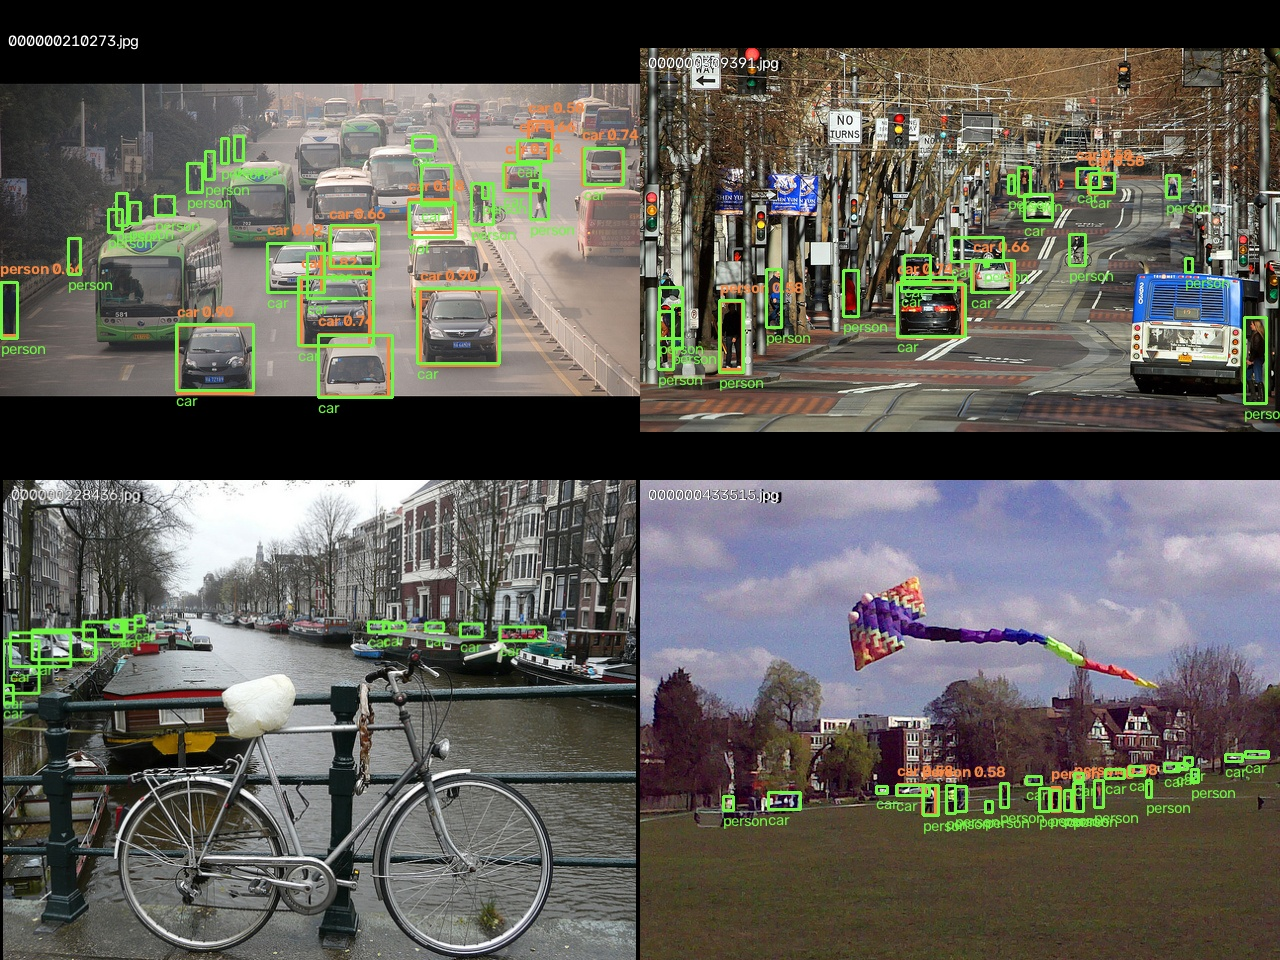
\includegraphics[width=0.9\textwidth]{figures/predictions_limites.jpg}
    \caption{Limite principale : les objets proches sont détectés, les
    petits objets lointains (piétons et voitures au fond, rive du canal,
    promeneurs sous le cerf-volant) sont largement manqués --- cohérent
    avec l'AP petits objets de 0,310 contre 0,652 pour les grands
    (section 5.6).}
    \end{figure}

    {\small Images COCO val2017 (Flickr, licences CC BY et CC BY-NC),
    identifiants 160864, 377588, 17207, 78823, 210273, 309391, 228436 et
    433515 ; générées avec
    \texttt{detection/src/04\_evaluate/visualize\_test\_predictions.py}.}

    
    \section{Bilan de la partie détection}
    
    Synthèse en une page du modèle finalement déployé (NanoDet-Plus-m-1.5x,
    896px, INT8 QDQ \texttt{u8s8}) :
    
    \begin{table}[!htbp]
    \centering
    \small
    \begin{adjustbox}{max width=\linewidth}
    \begin{tabular}{@{}ll@{}}
    \toprule
    \textbf{Indicateur} & \textbf{Valeur} \\
    \midrule
    Taille fichier (INT8) & 3,12 Mo (contrainte $\leq$ 5 Mo, 38\% de marge) \\
    mAP fp32 (\texttt{test.json}) & 0,485 \\
    mAP INT8 (\texttt{test.json}) & 0,462 \\
    Perte due à la quantification & -4,7\% \\
    IPS mesuré (CPU, INT8) & 26,9 (contrainte $\geq$ 25 IPS, $\sim$8\% de marge) \\
    \bottomrule
    \end{tabular}
    \end{adjustbox}
    \end{table}
    
    Les quatre contraintes dures du brief (full-CNN, quantifié INT8, taille
    $\leq$ 5 Mo, IPS $\geq$ 25) sont respectées. La progression sur trois générations
    (section 4) confirme empiriquement l'hypothèse posée dès la section 2.4
    : la résolution d'entrée profite spécifiquement aux petits objets
    (\texttt{AP\_small} +91,4\% entre 416px et 896px, de loin la métrique la
    plus transformée), et la toolchain de quantification développée en
    interne (section 5) ramène la perte due au passage en INT8 à -4,7\% sur
    le modèle final --- un résultat obtenu par une démarche itérative et
    mesurée (calibration \texttt{MinMax} d'abord, limites identifiées,
    \texttt{Percentile} ensuite) plutôt que par un choix de configuration
    pris au hasard.
    
    \textbf{Limites} :
    
    \begin{itemize}[leftmargin=1.5em]
      \item \textbf{Déséquilibre \texttt{person}/\texttt{car} jamais éliminé}
        --- le ratio de précision entre les deux classes se resserre au fil
        des générations (1,44 $\to$ 1,23, section 4.4) mais reste
        structurellement $>$1 à chaque génération, hérité d'un déséquilibre
        inhérent à COCO lui-même (section 3.2) que le sur-échantillonnage
        atténue sans l'annuler.
      \item \textbf{Petits objets toujours le point faible} --- malgré le
        gain le plus spectaculaire des trois générations,
        \texttt{AP\_small} (0,335 en fp32 à 896px) reste nettement en
        dessous d'\texttt{AP\_medium} (0,629) et \texttt{AP\_large} (0,684)
        : la hausse de résolution a réduit l'écart, pas comblé le désavantage
        structurel des petits objets.
      \item \textbf{Marge IPS qui se resserre avec la précision} --- 896px
        ne conserve que $\sim$8\% de marge sur le seuil de 25 IPS retenu
        (contre 400\% à 416px, section 6.2) : un compromis assumé, qui permet de rester au-delà du critère fixé à 25 IPS.
      \item \textbf{Mesures faites sur un poste de développement, pas une
        cible embarquée réelle} --- cohérent avec l'absence de contrainte
        matérielle dans le brief (section 1.1), mais les IPS et la mémoire
        rapportés ici resteraient à revalider sur le matériel embarqué
        final, dont les caractéristiques (CPU, présence ou non
        d'accélération INT8 dédiée) restent inconnues à ce stade.
      \item \textbf{Un seul split fixe, sans validation croisée} ---
        \texttt{train}/\texttt{val}/\texttt{test} proviennent d'un tirage
        aléatoire unique (graine fixée, section 3.1) : les chiffres rapportés
        sont ponctuels, sans intervalle de confiance ni estimation de leur
        variance à travers plusieurs tirages ou plusieurs seeds
        d'entraînement.
      \item \textbf{Écart de domaine COCO vs cas d'usage réel, non mesuré}
        --- COCO (section 3, choix motivé par la disponibilité de poids
        pré-entraînés sur ce même corpus) reste un ensemble de
        photographies grand public, pas des images de caméras de sécurité
        fixes. Les métriques rapportées dans ce rapport mesurent donc la
        performance sur la distribution COCO, pas directement sur le cas
        d'usage visé (section 1) --- un écart de domaine plausible, jamais
        quantifié empiriquement faute de données réelles de ce type
        disponibles pour ce projet.
    \end{itemize}
    
    
    \section{Suivi multi-objets et journalisation des événements}
    
    \subsection{Choix de la librairie et architecture générale}
    
    Le suivi (\emph{tracking}) s'appuie sur \texttt{ByteTrackTracker} du
    paquet \texttt{trackers} (successeur de \texttt{supervision.ByteTrack},
    déprécié depuis la version 0.28.0). Le rôle du tracker est de
    transformer des détections indépendantes d'un frame à l'autre en
    \textbf{pistes} porteuses d'un identifiant stable (\texttt{tracker\_id}) :
    condition nécessaire pour répondre à des requêtes comme « depuis combien
    de temps cette personne est-elle présente », qui exigent de savoir que
    la boîte vue au frame $t$ et celle vue au frame $t+1$ désignent le même
    objet.
    
    La librairie n'a \textbf{aucune notion de classe} en interne --- une
    seule instance partagée entre \texttt{person} et \texttt{car}
    associerait une détection \texttt{car} à une piste \texttt{person} par
    simple recouvrement géométrique (un piéton qui monte dans un véhicule,
    par exemple). \texttt{MultiClassByteTracker} (\texttt{agent/src/tracking/tracker.py})
    enveloppe donc \textbf{une instance de \texttt{ByteTrackTracker} par
    classe}, chacune allouant ses propres identifiants à partir de 0 --- un
    même entier \texttt{tracker\_id} peut donc désigner deux pistes
    différentes selon la classe, d'où l'usage systématique de la paire
    \texttt{(classe, tracker\_id)} comme clé partout où l'état est indexé
    (lissage, hystérésis, journal d'événements).

    \subsection{Paramètres retenus}

    Les valeurs retenues ont été validées empiriquement sur les sources
    vidéo de la démonstration, hors dataset COCO :
    
    \begin{table}[!htbp]
    \centering
    \small
    \begin{adjustbox}{max width=\linewidth}
    \begin{tabular}{@{}p{5.2cm}p{1.6cm}p{7.6cm}@{}}
    \toprule
    \textbf{Paramètre} & \textbf{Retenu} & \textbf{Justification} \\
    \midrule
    \texttt{track\_activation\_threshold} & \textbf{0,65} & Seuil (strict) pour \textbf{créer} une nouvelle piste --- abaissé pour un modèle aux scores plus modestes que ceux visés par défaut \\
    \texttt{high\_conf\_det\_threshold} & \textbf{0,35} & Seuil (permissif) qui route une détection vers l'association de 1\textsuperscript{re} passe plutôt que la 2\textsuperscript{e} (section 8.3) --- distinct du précédent, abaissé pour la même raison \\
    \texttt{lost\_track\_buffer} & \textbf{90} & Exprimé par la librairie en « frames à 30 FPS » mais utilisé en interne comme une tolérance en \textbf{secondes d'horloge réelle} (\texttt{maximum\_time\_without\_update = lost\_track\_buffer / 30.0}) --- voir discussion ci-dessous \\
    \texttt{minimum\_consecutive\_frames} & \textbf{5} & Nombre de mises à jour réussies consécutives avant qu'une piste reçoive un \texttt{tracker\_id} définitif --- relevé pour filtrer les créations de piste sur un faux positif isolé, sans trop retarder l'affichage (voir ci-dessous) \\
    \texttt{minimum\_iou\_threshold} & 0,1 (inchangé) & Seuil d'IoU minimal pour qu'une association détection$\leftrightarrow$piste soit retenue par l'algorithme d'assignation (8.3) \\
    \texttt{frame\_rate} & 30,0 (inchangé) & Voir mise en garde ci-dessous \\
    \bottomrule
    \end{tabular}
    \end{adjustbox}
    \end{table}
    
    Le choix de 90 pour \texttt{lost\_track\_buffer} (plutôt que le défaut
    30) porte la tolérance d'une piste perdue de 1 à 3 secondes réelles.
    Le tracker recevant l'horodatage de chaque frame, ce budget s'exprime
    en temps et non en nombre de frames : il ne dépend donc pas du débit
    réel de la démonstration, nettement inférieur à 30 FPS. Une seconde
    s'est révélée trop courte pour traverser une occlusion brève (piéton
    masqué par un véhicule, par exemple) sans que l'objet ne reparte avec
    un nouvel identifiant --- ce qui fausserait les comptages et les durées
    de présence du journal (section 8.4). Trois secondes conservent
    l'identifiant dans ces cas sans maintenir trop longtemps une piste
    réellement disparue.

    Le paramètre \texttt{minimum\_consecutive\_frames} fixe le délai avant
    qu'un nouvel objet apparaisse à l'écran : une piste doit être associée
    pendant ce nombre de frames d'affilée, et une piste pas encore confirmée est
    supprimée au premier raté du détecteur. Une première valeur de 15
    retardait visiblement l'affichage. Le tracker a été rejoué sur les 4
    vidéos de démo (1\,600 frames, au débit réel de la démonstration,
    $\sim$18 FPS) avec plusieurs valeurs :

    \begin{table}[!htbp]
    \centering
    \small
    \begin{adjustbox}{max width=\linewidth}
    \begin{tabular}{@{}lcccc@{}}
    \toprule
    \texttt{minimum\_consecutive\_frames} & \textbf{Délai médian} & \textbf{Délai p90} & \textbf{Détections nettes affichées} & \textbf{Pistes éphémères} \\
    \midrule
    15 & 0,94 s & 1,28 s & 91\,\% & 1 \\
    8 & 0,56 s & 0,98 s & 95\,\% & 0 \\
    \textbf{5 (retenu)} & \textbf{0,39 s} & \textbf{0,80 s} & \textbf{97\,\%} & \textbf{1} \\
    3 & 0,28 s & 0,69 s & 98\,\% & 1 \\
    \bottomrule
    \end{tabular}
    \end{adjustbox}
    \end{table}

    Le délai est mesuré entre le début de la suite continue de détections
    d'un objet et son premier affichage ; une piste est dite éphémère si
    elle reste affichée moins de 0,5 s. Passer de 15 à 5 divise le délai
    par 2,4 sans faire apparaître de faux positifs supplémentaires (53 puis
    54 pistes au total). 3 serait un peu plus rapide mais laisse moins de
    marge sur des scènes plus difficiles. Le seuil de création
    \texttt{track\_activation\_threshold} n'est pas en cause : les scores
    du modèle INT8 vont par paliers (0,576, 0,658, 0,740\ldots), et 0,65
    ou 0,60 donnent exactement le même résultat.

    \subsection{Logique de traitement, frame par frame}
    
    \subsubsection{Association détection$\leftrightarrow$piste (dans \texttt{ByteTrackTracker})}
    
    À chaque appel de \texttt{update()}, pour chaque classe indépendamment :
    
    \begin{enumerate}[leftmargin=1.7em]
      \item \textbf{Prédiction} --- l'état (position, vitesse) de chaque
        piste existante est avancé d'un pas par son filtre de Kalman
        interne, calibré sur le temps réellement écoulé depuis la dernière
        mise à jour (pas un pas fixe par frame).
      \item \textbf{Élagage préliminaire} --- les pistes ayant dépassé leur
        budget de temps sans association sont retirées avant l'association,
        pour ne pas polluer l'étape suivante avec des candidats déjà morts.
      \item \textbf{Séparation des détections par confiance} --- les
        détections du frame sont scindées en deux lots selon
        \texttt{high\_conf\_det\_threshold} : confiance haute et confiance
        basse.
      \item \textbf{Association, 1\textsuperscript{re} passe (confiance haute)} ---
        toutes les pistes existantes (prédites) sont mises en correspondance
        avec les détections de confiance haute par un algorithme
        d'assignation optimal (\texttt{scipy.optimize.linear\_sum\_assignment},
        maximisation de l'IoU --- une version sans initialisation de
        l'algorithme hongrois), une association n'étant retenue que si son
        IoU dépasse \texttt{minimum\_iou\_threshold}.
      \item \textbf{Association, 2\textsuperscript{e} passe (confiance basse)} --- les
        pistes \textbf{encore non associées} après la 1\textsuperscript{re} passe
        tentent une seconde association, cette fois avec les détections de
        confiance basse --- c'est le principe central de ByteTrack : une
        détection de faible confiance peut malgré tout confirmer une piste
        déjà établie (typiquement une occlusion partielle), sans jamais
        pouvoir en créer une nouvelle.
      \item \textbf{Confirmation de piste} --- une piste associée (l'une ou
        l'autre passe) ne reçoit un \texttt{tracker\_id} définitif que si
        elle cumule au moins \texttt{minimum\_consecutive\_frames} mises à
        jour réussies \textbf{consécutives} ; avant ce seuil, elle existe en
        interne mais ressort avec \texttt{tracker\_id=-1}.
      \item \textbf{Création de nouvelles pistes} --- seules les détections
        de confiance haute encore non associées après la 1\textsuperscript{re} passe
        \textbf{et} dont la confiance dépasse
        \texttt{track\_activation\_threshold} (plus strict que
        \texttt{high\_conf\_det\_threshold}) donnent naissance à une
        nouvelle piste. Les détections de confiance basse non associées ne
        créent jamais de piste.
      \item \textbf{Élagage final} --- toute piste à la fois immature (pas
        encore confirmée) et non associée ce frame-ci, ou ayant dépassé son
        budget de temps sans association (\texttt{lost\_track\_buffer}), est
        retirée de la liste.
    \end{enumerate}
    
    Point notable : \texttt{track\_activation\_threshold} et
    \texttt{high\_conf\_det\_threshold} jouent des rôles distincts
    (0,65 et 0,35 retenus) --- le premier gouverne
    uniquement la \textbf{naissance} d'une piste, le second gouverne
    uniquement quelles détections tentent la 1\textsuperscript{re} passe d'association.
    Une confusion entre les deux mènerait soit à des pistes trop faciles à
    créer (bruit), soit à des pistes établies perdues trop facilement sur
    une simple occlusion partielle.
    
    \subsubsection{Post-traitement (dans \texttt{MultiClassByteTracker})}
    
    Quatre mécanismes supplémentaires sont appliqués \textbf{après} le
    tracker de base, par piste confirmée --- tous centralisés dans
    \texttt{config/tracker.yaml} (comme \texttt{tracker\_kwargs} ci-dessus),
    sans équivalent dans la librairie \texttt{trackers} elle-même :
    
    \begin{itemize}[leftmargin=1.5em]
      \item \textbf{Lissage} --- moyenne mobile exponentielle
        ($\alpha=$\texttt{smoothing\_alpha}$=0,55$) sur les coordonnées de
        boîte affichées, indexée par \texttt{(classe, tracker\_id)} : réduit
        la gigue visuelle d'une détection à l'autre sans introduire un
        retard excessif sur le mouvement réel. Le lissage étant appliqué une
        fois par frame, sa constante de temps dépend du débit : la valeur
        nominale 0,4, pensée pour 30 FPS, aurait rendu le lissage environ
        1,7 fois plus lent au débit réel de la démonstration ($\sim$18 FPS,
        section 8.2). 0,55 rétablit approximativement la réactivité visée.
      \item \textbf{Hystérésis d'affichage} (trigger de Schmitt) --- une
        piste doit dépasser \texttt{hysteresis\_high}$=0,4$ pour devenir
        visible, mais ne redevient invisible qu'en repassant sous
        \texttt{hysteresis\_low}$=0,2$ (pas simplement sous
        \texttt{hysteresis\_high} à nouveau) --- évite qu'un score oscillant
        juste autour d'un seuil unique fasse clignoter la boîte d'un frame à
        l'autre. La détection qui fait repasser une piste visible sous
        \texttt{hysteresis\_low} est encore renvoyée une fois, marquée
        \texttt{origin="weak"}, et affichée en pointillés plutôt que de
        disparaître brutalement. Un score déjà filtré en amont (ex. seuil
        de score des scripts de démo) devient ainsi redondant pour tout ce
        qui sort d'ici : c'est déjà une boîte destinée à être affichée.
      \item \textbf{Extrapolation (« coasting »)} --- une piste confirmée,
        non ré-associée à une détection ce frame-ci mais toujours dans sa
        fenêtre de tolérance interne, est quand même renvoyée, marquée
        \texttt{origin="predicted"}, avec une position lue directement sur
        l'état du filtre de Kalman (\texttt{track.get\_state\_bbox()}) ---
        un accès à l'état interne de la librairie, non exposé par l'API
        publique \texttt{.update()}, seul moyen d'obtenir cette
        extrapolation. Réservé aux pistes déjà devenues visibles au moins
        une fois. Ces positions prédites sont calculées mais \textbf{ne sont
        pas affichées} par les scripts de démonstration actuels, qui ne
        dessinent que des boîtes adossées à une détection réelle.
      \item \textbf{Budget de coasting cumulé} ---
        \texttt{max\_cumulative\_predicted\_seconds}$=3,0$s : contrairement
        à \texttt{lost\_track\_buffer} (section 8.2), qui plafonne chaque
        \emph{épisode individuel} de coasting, ce budget plafonne le
        \textbf{cumul} sur toute la durée de vie d'une piste. Sans lui, une
        piste chroniquement à la limite (détections intermittentes qui la
        ramènent juste avant expiration, sans jamais la confirmer
        franchement) pourrait fantômer indéfiniment, épisode après épisode.
        Remis à zéro uniquement quand la piste repasse par une confirmation
        solide (score $\geq$ \texttt{hysteresis\_high}) --- même ordre de
        grandeur que \texttt{lost\_track\_buffer} par cohérence d'intention,
        appliqué ici au cumul plutôt qu'à un seul épisode.
    \end{itemize}
    
    \textbf{Invariant central} : chaque boîte renvoyée porte, en plus de son
    \texttt{tracker\_id}, un indicateur \texttt{is\_coasted} et une origine.
    \texttt{is\_coasted=False} (\texttt{origin="confirmed"}) désigne une
    détection sûre, affichée en trait plein ; \texttt{is\_coasted=True}
    regroupe les boîtes non fiables : détection faible d'une piste visible
    (\texttt{"weak"}, affichée en pointillés, \texttt{draw\_dashed\_rect})
    et position seulement prédite (\texttt{"predicted"}, non affichée).
    Aucune boîte \texttt{is\_coasted} ne doit être transmise au journal
    d'événements (8.4) comme une observation réelle, sous peine de faire
    « tourner le temps » d'une piste sur une simple prédiction de
    mouvement. Cet invariant est appliqué à l'appel du journal via une
    fonction \texttt{confirmed\_only()} qui écarte ces boîtes avant tout
    appel à \texttt{EventStore.update()}, dans le script de démonstration
    qui combine tracking et journalisation (\texttt{03\_live\_agent\_demo.py}).
    
    Enfin, à chaque frame, l'état de lissage et d'hystérésis des pistes
    définitivement abandonnées par le tracker (au-delà de
    \texttt{lost\_track\_buffer}) est purgé --- sans quoi une démonstration
    tournant longtemps accumulerait indéfiniment de l'état mort en mémoire.
    
    \subsection{Journalisation des événements (\texttt{EventStore})}
    
    \subsubsection{Schéma et choix de conception}
    
    Le journal (\texttt{agent/src/journal/event\_store.py}) est une base
    \textbf{SQLite} avec trois tables :
    
    \begin{table}[!htbp]
    \centering
    \footnotesize
    \begin{adjustbox}{max width=\linewidth}
    \begin{tabular}{@{}lp{7.5cm}p{6.5cm}@{}}
    \toprule
    \textbf{Table} & \textbf{Colonnes} & \textbf{Rôle} \\
    \midrule
    \texttt{events} & \texttt{track\_id}, \texttt{class}, \texttt{first\_seen}, \texttt{last\_seen} & Une ligne par piste vue au moins une fois \\
    \texttt{alerts} & \texttt{alert\_type}, \texttt{object\_class}, \texttt{zone\_name}, \texttt{threshold\_seconds}, \texttt{person\_threshold}, \texttt{car\_threshold}, \texttt{count\_threshold}, \texttt{window\_minutes}, \texttt{created\_at} & Une ligne par règle configurée, 4 types hétérogènes (\texttt{duration}/\texttt{co\_occurrence}/\texttt{surge}/\texttt{zone}, section 9.5) dans une table à colonnes creuses --- chaque type ne renseigne que les colonnes qui le concernent \\
    \texttt{zone\_events} & \texttt{id}, \texttt{zone\_name}, \texttt{class}, \texttt{track\_id}, \texttt{entered\_at} & Une ligne par \textbf{entrée} en zone (transition dehors$\to$dedans détectée par \texttt{ZoneMonitor}, \texttt{agent/src/alerts/zones.py}), pas une ligne par frame passé dedans \\
    \bottomrule
    \end{tabular}
    \end{adjustbox}
    \end{table}
    
    \texttt{alerts} utilise une clé composite \texttt{(alert\_type,
    object\_class, zone\_name)}, avec chaîne vide \texttt{''} (jamais
    \texttt{NULL}) comme sentinelle pour les colonnes non pertinentes à un
    type donné --- SQLite ne fait jamais collisionner deux \texttt{NULL}
    dans une contrainte \texttt{UNIQUE}, donc des \texttt{NULL} en
    sentinelle auraient laissé s'accumuler plusieurs règles du même type au
    lieu de la remplacer (\texttt{ON CONFLICT} ne se déclenchant jamais
    entre deux \texttt{NULL}).
    
    La clé primaire de \texttt{events} est le couple \texttt{(class,
    track\_id)} --- cohérent avec l'espace de \texttt{tracker\_id} propre à
    chaque classe déjà signalé en 8.1. Chaque frame où une piste est vue
    déclenche un \emph{upsert} (\texttt{INSERT ... ON CONFLICT(class,
    track\_id) DO UPDATE SET last\_seen = excluded.last\_seen}) : la ligne
    est créée à la première apparition, puis seule \texttt{last\_seen} est
    rafraîchie ensuite.
    
    Choix de conception notable : il n'existe \textbf{aucun champ
    « actif »} stocké. Une piste est considérée active si
    \texttt{last\_seen} est récent (paramètre
    \texttt{active\_within\_seconds}), pas via un état à mettre à jour
    explicitement. Ce choix évite d'avoir à décider frame par frame si une
    piste doit être marquée « terminée » --- décision déjà prise, en
    pratique, par le tracker lui-même (section 8.3) : une piste peut
    réapparaître avec le même \texttt{tracker\_id} après une brève absence
    tant qu'elle reste dans la fenêtre de tolérance de
    \texttt{lost\_track\_buffer}, ce que la seule récence de
    \texttt{last\_seen} reflète directement, sans double comptabilité à
    synchroniser entre le tracker et le journal.
    
    \subsubsection{Accès concurrent}
    
    Le journal est accédé depuis deux threads distincts dans le système
    complet : la boucle vidéo (tracking, écriture) d'un côté, le thread de
    l'agent conversationnel (lecture, en réponse à une requête utilisateur)
    de l'autre. La connexion SQLite est ouverte avec
    \texttt{check\_same\_thread=False}, associée à un
    \texttt{threading.Lock} explicite posé autour de \textbf{chaque} accès
    à la connexion --- la sérialisation des lectures/écritures est ainsi
    assurée nous-mêmes plutôt que de compter sur un comportement implicite
    du module \texttt{sqlite3}. Point d'implémentation à noter :
    \texttt{active\_durations()} délègue entièrement à
    \texttt{active\_tracks()} (qui verrouille déjà) \textbf{sans} reprendre
    le verrou lui-même --- un \texttt{threading.Lock} standard n'étant pas
    réentrant, un second verrouillage depuis le même thread y
    provoquerait un interblocage.
    
    \subsubsection{Requêtes exposées}
    
    Huit méthodes d'accès au journal --- la table \texttt{events} seule
    pour les six premières, \texttt{zone\_events} pour les deux dernières.
    Six d'entre elles servent directement les tools de l'agent (section
    9.5) ; \texttt{active\_durations} et \texttt{log\_zone\_entry} sont
    appelées par les moniteurs d'alerte et de zone :
    
    \begin{itemize}[leftmargin=1.5em]
      \item \texttt{count\_between(classe, début, fin)} --- nombre de
        pistes distinctes de cette classe dont la \textbf{première}
        apparition tombe dans l'intervalle. Répond à « combien de voitures
        sont passées entre 12h15 et 12h30 » (\texttt{count\_between}), et
        sert aussi de base à \texttt{count\_total} (borne de fin =
        maintenant).
      \item \texttt{active\_tracks(classe, active\_within\_seconds)} ---
        pistes vues il y a moins de \texttt{active\_within\_seconds}.
        Répond à « combien de véhicules sont dans le champ maintenant »
        (\texttt{count\_now}).
      \item \texttt{active\_durations(classe, active\_within\_seconds)} ---
        pour chaque piste active, la durée écoulée depuis sa
        \textbf{première} apparition. Répond à « personne présente depuis
        plus de 10 secondes » (consommé par \texttt{AlertMonitor}, section
        9.9, pas directement par un tool).
      \item \texttt{most\_recent\_last\_seen(classe)} --- timestamp de la
        dernière détection, toutes pistes confondues. Répond à « quand la
        dernière voiture est-elle passée » (\texttt{time\_since\_last\_seen}).
        La dernière \emph{détection} et non la dernière \emph{apparition} :
        une voiture présente depuis une minute est toujours visible.
      \item \texttt{average\_presence\_duration(classe)} --- durée moyenne
        (\texttt{last\_seen} $-$ \texttt{first\_seen}) sur toutes les pistes
        de cette classe depuis le début de la session. Répond à « en
        moyenne combien de temps reste une personne »
        (\texttt{average\_presence\_duration}).
      \item \texttt{peak\_concurrent\_count(classe)} --- nombre maximal de
        pistes actives \textbf{simultanément} à un instant quelconque
        depuis le début de la session. Répond à « quel a été le pic de
        véhicules » (\texttt{peak\_concurrent\_count}).
      \item \texttt{log\_zone\_entry(zone, classe, track\_id)} --- écrit
        une ligne dans \texttt{zone\_events} ; appelée par
        \texttt{ZoneMonitor} à chaque entrée détectée, jamais directement
        par un tool.
      \item \texttt{count\_zone\_entries(zone, classe)} --- nombre
        d'entrées journalisées dans cette zone. Répond à « combien de fois
        une personne est entrée dans la zone centrale »
        (\texttt{count\_zone\_entries}).
    \end{itemize}
    
    Les méthodes basées sur une fraîcheur (\texttt{active\_tracks},
    \texttt{active\_durations}) utilisent volontairement une tolérance
    \textbf{courte} par défaut (1 seconde). Cette tolérance ne compense
    \textbf{aucune latence d'exécution} (voir section 9.7 pour la
    démonstration) : elle absorbe uniquement le clignotement occasionnel du
    détecteur (quelques frames ratées sur un objet pourtant toujours
    présent). C'est une question produit à part entière, pas un simple
    délai technique à deviner. Les tools de l'agent (\texttt{count\_now},
    \texttt{time\_since\_last\_seen}) utilisent une tolérance un peu plus
    large, 2 secondes (\texttt{freshness\_seconds},
    \texttt{config/agent.yaml}), tandis que \texttt{AlertMonitor} conserve
    la valeur par défaut.

    \section{Agent conversationnel}
    
    L'agent répond en langage naturel aux questions portant sur les
    détections journalisées en section 8 --- compter les objets présents,
    filtrer par plage horaire, configurer une alerte de présence continue, etc...
    (cahier des charges, section 1.1). Deux composants : les \textbf{tools}
    qui font le pont entre une question et une requête sur
    \texttt{EventStore} (\texttt{agent/src/agent/tools.py}), et la
    \textbf{boucle agent} qui orchestre l'appel au LLM et l'exécution des
    tools qu'il demande (\texttt{agent/src/agent/agent.py}).
    
    \subsection{Choix du runtime et critères de sélection}
    
    Le runtime retenu est \texttt{llama.cpp} directement, plutôt
    qu'Ollama --- qui l'utilise de toute façon en interne pour un usage
    mono-utilisateur local, la différence sous le capot est marginale. Ce choix est cohérence avec la philosophie déjà suivie côté
    détection (\texttt{onnxruntime} plutôt que PyTorch complet en
    déploiement, section 5) --- un moteur d'inférence C++ léger, sans
    dépendance à un framework d'entraînement, pour le LLM comme pour la
    détection.
    
    Le choix du modèle lui-même répond à des critères explicites, dans le
    même esprit méthodologique que la sélection d'architecture de
    détection (section 2.2) :
    
    \begin{itemize}[leftmargin=1.5em]
      \item \textbf{Handler de tool-calling natif dans \texttt{llama.cpp}}
        --- un parseur dédié au format d'appel de tools du modèle, plus
        fiable que le \emph{fallback} générique\footnote{Liste officielle
        des formats de tool-calling supportés :
        \texttt{docs/function-calling.md}, dépôt
        \texttt{ggml-org/llama.cpp}.}. Critère éliminatoire, comme le «
        graphe exporté propre » l'était pour l'architecture de détection.
      \item \textbf{Licence compatible avec un usage en entreprise} ---
        même raisonnement que l'exclusion de YOLOv8n en AGPL-3.0
        (section 2.2) : un modèle sous licence non-commerciale est écarté
        quel que soit son mérite technique.
      \item \textbf{Budget VRAM disponible} --- 8 Go sur la RTX 4060 déjà
        utilisée pour l'entraînement (section 4), à ne pas saturer.
      \item \textbf{Validation empirique par un banc de test dédié} plutôt
        que par un chiffre proxy : contrairement au mAP COCO pour la
        détection (section 2.4), il n'existe pas de benchmark public
        directement transférable à \emph{notre} jeu de 12 tools --- la
        seule mesure fiable est un banc de test construit sur mesure
        (section 9.3).
    \end{itemize}
    
    \subsection{Comparatif étendu des modèles candidats}
    \label{sec:agent-comparatif}
    
    \begin{landscape}
    \begin{table}[p]
    \centering
    \footnotesize
    \renewcommand{\arraystretch}{1.25}
    \begin{adjustbox}{max width=\linewidth}
    \begin{tabular}{@{}p{3.6cm}p{1.2cm}p{2.0cm}p{2.4cm}p{2.0cm}p{3.4cm}p{7.0cm}@{}}
    \toprule
    \textbf{Modèle} & \textbf{Params} & \textbf{Taille Q4\_K\_M} & \textbf{VRAM totale estimée\textsuperscript{*}} & \textbf{Marge/8 Go} & \textbf{Licence} & \textbf{Remarque} \\
    \midrule
    Qwen2.5-7B-Instruct & 7B & 4,68 Go (confirmé) & $\sim$5,5--6 Go & confortable & Apache 2.0 & Référence connue, déjà validée de bout en bout avant ce comparatif étendu \\
    Hermes-3-Llama-3.1-8B (Nous Research) & 8B & 4,92 Go (confirmé) & $\sim$5,7--6,2 Go & confortable & Communautaire Llama 3.1 (héritée) & Format de tool-call (Hermes) réputé fiable en JSON structuré \\
    Functionary-small-v3.2 (MeetKai) & 8B & 4,92 Go (bartowski) / 4,66 Go en Q4\_0 (dépôt officiel, seul quant. dispo) & $\sim$5,7--6,2 Go & confortable & Communautaire Llama 3.1 (héritée, base Llama-3.1-8B) & Seul modèle conçu exclusivement pour le tool-calling, mais support des appels \textbf{parallèles} cassé côté \texttt{llama.cpp} (section 9.3.3) \\
    Command R7B (Cohere) & $\sim$8B & 5,06 Go (confirmé) & $\sim$5,9--6,4 Go & confortable & \textbf{CC-BY-NC} (non-commercial) & Écarté sans test --- même raisonnement que l'exclusion AGPL de YOLOv8n (section 2.2) \\
    \textbf{Granite-4.1-3B (IBM)} & 3B & 2,10 Go (confirmé) & $\sim$2,8--3,3 Go & très large & Apache 2.0 & Beaucoup plus rapide, marge VRAM énorme --- capacité de raisonnement sur l'extraction de paramètres fins à valider empiriquement \\
    Mistral-Nemo-Instruct-2407 & 12B & 7,48 Go (confirmé) & $\sim$8,3--8,8 Go & \textbf{dépasse 8 Go} & Apache 2.0 & Écarté sans test --- seul candidat dépassant le budget VRAM mesuré \\
    \bottomrule
    \end{tabular}
    \end{adjustbox}
    
    \vspace{0.6em}
    \raggedright
    \textit{\footnotesize\textsuperscript{*} VRAM totale = poids + KV-cache/overhead runtime, estimée selon le
    même ratio que la mesure réelle de Qwen2.5-7B (4,68$\to\sim$5,5--6 Go) ---
    à confirmer par mesure directe pour chaque nouveau candidat, pas une
    valeur garantie a priori.}
    \end{table}
    \end{landscape}
    
    Sur les 6 candidats, 2 sont écartés sans même être testés : Command
    R7B sur un critère non technique (licence CC-BY-NC), Mistral-Nemo
    parce qu'il dépasse seul le budget VRAM mesuré de 8 Go, sans laisser de
    marge pour le KV-cache. \textbf{Les 4 candidats restants sont soumis à
    un banc de test réel} (section 9.3) --- Qwen2.5-7B-Instruct, Hermes-3-Llama-3.1-8B,
    Functionary-small-v3.2 et Granite-4.1-3B.
    
    \subsection{Banc de test réel}
    
    \subsubsection{Méthodologie}
    
    Une banque de \textbf{36
    questions} (\texttt{cases.py}) couvrant les 12 tools exposés (section 9.5) ainsi que des variantes et pièges délibérés --- synonymes,
    formulation en anglais, désambiguïsation « maintenant » vs « total »,
    horaires absolus et relatifs, appels multiples dans un même tour, zone
    inconnue, questions hors périmètre.
    Chaque question est rejouée
    \textbf{10 fois} --- la sortie d'un LLM n'est pas déterministe d'un tick
    à l'autre (sampling). Un cas qui échoue une fois sur dix n'est pas
    équivalent à un cas qui échoue toujours.
    
    Le prompt système utilisé est \textbf{celui de la production}
    (\texttt{config/agent.yaml}, chargé dynamiquement, jamais recopié en
    dur dans le banc de test) --- pour ne jamais valider un prompt
    différent de celui réellement déployé. Le scoring
    (\texttt{harness.py:score\_case}) est \textbf{strict} : appariement
    glouton, indépendant de l'ordre, entre les appels de tools attendus et
    les appels réellement effectués (nom + arguments) ; un cas n'est
    compté « réussi » que si \textbf{tous} les appels attendus sont
    retrouvés \textbf{et} qu'\textbf{aucun} appel superflu ne reste --- un
    tool de trop (ex. compter les deux classes quand une seule était
    demandée) est une vraie erreur de comportement. .
    
    \subsubsection{Résultats agrégés}
    
    \begin{table}[!htbp]
    \centering
    \small
    \begin{adjustbox}{max width=\linewidth}
    \begin{tabular}{@{}lcccc@{}}
    \toprule
    \textbf{Modèle} & \textbf{Taux de réussite} & \textbf{Latence médiane} & \textbf{Latence P95} & \textbf{VRAM confirmée} \\
    \midrule
    \textbf{Granite-4.1-3B} & \textbf{97,2\%} & \textbf{0,65 s} & \textbf{1,01 s} & \textbf{2,10 Go} \\
    Hermes-3-Llama-3.1-8B & 93,9\% & 1,13 s & 1,58 s & 4,92 Go \\
    Qwen2.5-7B-Instruct & 92,8\% & 1,24 s & 2,03 s & 4,68 Go \\
    Functionary-small-v3.2 & 90,6\% & 1,03 s & 1,94 s & 4,66 Go \\
    \bottomrule
    \end{tabular}
    \end{adjustbox}
    
    \vspace{0.4em}
    \raggedright
    \textit{\footnotesize Chiffres finaux, \textbf{10 répétitions par cas} (360 exécutions par modèle).}
    \end{table}
    
    Granite-4.1-3B se distingue nettement sur les trois axes mesurés :
    meilleur taux de réussite (97,2\%), latence médiane la plus basse
    (0,65 s, $\sim$2$\times$ plus rapide que les trois autres) et empreinte
    VRAM la plus faible (2,10 Go). Hermes-3 et Qwen2.5-7B se tiennent proches
    en précision (93,9\% et 92,8\%) mais restent nettement plus lents et plus
    lourds. Functionary-small-v3.2 termine dernier sur les trois métriques
    --- sa latence mesurée est en outre faussée à la baisse par des échecs
    précoces et fréquents (section 9.3.3), donc probablement plus optimiste
    que sa latence réelle sur un échange qui aboutit normalement.
    
    \subsubsection{Analyse des échecs}
    
    Erreurs restantes, propres à chaque modèle, confirmées sur
    l'échantillon à 10 répétitions :
    
    \begin{itemize}[leftmargin=1.5em]
      \item \textbf{Qwen2.5-7B} : convertit systématiquement « midi » en
        \texttt{13:00}/\texttt{13:15} au lieu de \texttt{12:00}/\texttt{12:15}
        sur 2 cas indépendants (\texttt{count\_since\_\_loose\_natural\_phrasing},
        0/10 ; \texttt{count\_between\_\_morning}, 2/10) --- une erreur de
        compréhension déterministe, pas de la formulation non standard.
        Surtout, sur \texttt{multi\_\_compare\_now} (2 appels nécessaires),
        \textbf{7/10 runs partent en boucle} (40 à 49 appels
        \texttt{count\_now} alternés sans converger vers une réponse), dont
        \textbf{3 font planter le serveur} (JSON d'arguments malformé côté
        \texttt{llama.cpp}) --- ce que l'échantillon à 3 répétitions ne
        laissait voir que comme un cas isolé se révèle être le comportement
        \textbf{majoritaire} de Qwen sur ce cas précis.
      \item \textbf{Hermes-3-8B} : confond systématiquement « depuis 9h du
        matin » (heure absolue) avec « il y a 9 minutes »
        (\texttt{minutes\_ago: 9}, 8/10) --- erreur de compréhension plus
        grave que celle de Qwen sur un cas du même type. Flou sur les
        formulations temporelles relatives (« cette dernière demi-heure »,
        6/10 ; « midi et quart », 7/10, parfois interprété comme une durée
        relative erronée). Sur \texttt{multi\_\_compare\_now}, 6/10 runs
        corrects ; les 4 échecs ajoutent un appel \texttt{count\_now}
        redondant plutôt que de partir en boucle incontrôlée --- une
        dérive contenue, sans commune mesure avec celle de Qwen sur le même
        cas.
      \item \textbf{Granite-4.1-3B} : confirmé comme le point faible
        principal, « cette dernière demi-heure » ne passe que \textbf{3/10}
        --- le modèle glisse vers un horaire absolu \emph{inventé} plutôt
        que d'utiliser \texttt{minutes\_ago}, avec des valeurs qui varient
        d'un run à l'autre (\texttt{10:00}, \texttt{13:30}, \texttt{15:00}...),
        signe qu'il n'a pas de référence fiable à « maintenant » pour ce
        type de formulation. C'est nettement plus fréquent que ne le
        suggérait l'échantillon à 3 répétitions (2/3). En dehors de ce cas,
        \textbf{aucune autre erreur} sur les 35 cas restants.
      \item \textbf{Functionary-small-v3.2} : le moins fiable des 4 sur cet
        échantillon élargi. Confond systématiquement une alerte de durée de
        présence en anglais avec une alerte de seuil
        (\texttt{set\_surge\_alert} au lieu de
        \texttt{set\_presence\_duration\_alert}, 9/10). Le crash de
        grammaire déjà documenté sur \texttt{multi\_\_compare\_now}
        (section 9.3.1) se confirme \textbf{beaucoup plus fréquent}
        qu'estimé sur 3 répétitions : \textbf{9/10 runs plantent le
        serveur}, pas un cas isolé. Deux cas auparavant propres deviennent
        légèrement flaky sur l'échantillon élargi
        (\texttt{time\_since\_last\_seen\_\_car} 9/10,
        \texttt{peak\_concurrent\_count\_\_car} 8/10). \textbf{Nuance de
        mesure} : sur \texttt{count\_between\_\_morning} (6/10), les échecs
        viennent en partie d'un horaire rendu \texttt{"8:00"} plutôt que
        \texttt{"08:00"} attendu par le scoring strict (section 9.3.1) ---
        une réponse sémantiquement correcte mais pénalisée par
        l'appariement exact, à distinguer d'une vraie erreur de
        raisonnement.
    \end{itemize}
    
    \subsection{Décision finale : modèle retenu}
    
    \textbf{Granite-4.1-3B est retenu}. Premièrement la détection tourne exclusivement sur CPU en déploiement
    (\texttt{CPUExecutionProvider}, section 6.2) --- elle ne consomme donc
    pas de VRAM à proprement parler. Mais le script de démo complet
    (\texttt{demo/src/scripts/03\_live\_agent\_demo.py}) fait tourner le pipeline
    vidéo (capture, tracking, journal, rendu \texttt{cv2.imshow}) et le
    serveur LLM \textbf{en parallèle, sur la même machine}, équipée d'un
    \textbf{unique GPU} (RTX 4060, 8 Go) --- la seule ressource GPU
    disponible ce jour-là doit donc absorber non seulement le serveur LLM,
    mais aussi tout ce qui tourne par ailleurs sur ce même poste pendant
    une présentation en direct (partage d'écran ou enregistrement,
    compositeur du bureau, navigateur). Avec Qwen2.5-7B ou Hermes-3-8B
    (4,68--4,92 Go de poids seuls, $\sim$5,5--6,2 Go une fois le KV-cache
    compté), la marge restante sur 8 Go est confortable en isolation mais
    se resserre vite dès que d'autres processus sollicitent le GPU.
    \textbf{Granite-4.1-3B (2,10 Go de poids, $\sim$2,8--3,3 Go au total)
    libère 2,5 à 3 Go de VRAM supplémentaires} --- une marge de sécurité
    réelle.
    Ensuite Granite obtient \textbf{97,2\%}, le \textbf{meilleur taux de
    réussite confirmé des 4 candidats}. Granite reste par ailleurs
    \textbf{$\sim$2$\times$ plus rapide} que tous les autres (médiane
    0,65 s contre 1,03--1,24 s). Ce gain de vitesse compte directement pour
    ce genre de projet où la latence entre la requête et la réponse de l'agent peut entraîner des conflits sur la fraîcheur des données. La section 9.7 traite de ce risque dès la
    conception. Son
    principal point faible confirmé (formulations temporelles relatives
    floues, 3/10 sur « cette dernière demi-heure », section 9.3.3) reste
    une erreur de sélection d'argument, pas une erreur de compréhension
    temporelle grave comme celle d'Hermes sur « 9h du matin » ni une
    instabilité structurelle comme les boucles incontrôlées de Qwen sur
    \texttt{multi\_\_compare\_now} (7/10 runs, dont 3 crashs serveur) ---
    un type d'erreur plus inquiétant pour un usage produit réel. Licence
    Apache 2.0, et aucun patch de template nécessaire (contrairement à
    Hermes/Functionary).
    
    \subsection{Les tools }
    
    12 tools, tous généralisés par
    \texttt{object\_class} (\texttt{"person"} ou \texttt{"car"}) plutôt que
    dupliqués par classe, regroupés en 3 catégories
    (\texttt{agent/src/agent/tool\_schemas.py}) :
    
    \begin{itemize}[leftmargin=1.5em]
      \item \textbf{Comptage} --- \texttt{count\_now} (présents
        actuellement), \texttt{count\_total} (distincts depuis le début de
        la session), \texttt{count\_since} (depuis un point de départ,
        heure absolue \emph{ou} durée relative), \texttt{count\_between}
        (entre deux horaires précis).
      \item \textbf{Statistiques dérivées} --- \texttt{time\_since\_last\_seen}
        (délai depuis la dernière détection : le nombre de secondes, ou,
        si un objet est visible, une phrase déjà rédigée ; à partir d'un
        délai de 0, Granite concluait « aucune voiture visible » 10 fois
        sur 10), \texttt{average\_presence\_duration}
        (durée moyenne de présence), \texttt{peak\_concurrent\_count} (pic
        d'objets simultanés).
      \item \textbf{Alertes (configuration uniquement)} ---
        \texttt{set\_presence\_duration\_alert} (présence continue trop
        longue), \texttt{set\_co\_occurrence\_alert} (seuils combinés
        personnes ET véhicules), \texttt{set\_surge\_alert} (afflux/rafale
        en fenêtre glissante), \texttt{set\_zone\_alert} et
        \texttt{count\_zone\_entries} (zones de danger prédéfinies). Ces tools
        n'exécutent pas eux-mêmes la surveillance de la condition, rôle du
        mécanisme d'alerte (\texttt{agent/src/alerts/alerts.py}).
    \end{itemize}
    
    \subsection{Boucle agent et function-calling}
    
    \texttt{Agent.ask()} envoie la question au serveur
    (\texttt{chat.completions.create}) avec un
    prompt système en français et la liste des tools disponibles. Deux
    issues possibles à chaque tour : soit le serveur renvoie directement une
    réponse textuelle (fin de boucle), soit il renvoie un ou plusieurs
    \texttt{tool\_calls}. Dans ce second cas, chaque appel passe par une
    table de dispatch (nom de tool $\to$ méthode Python réelle),
    volontairement protégée : toute exception levée par un tool est
    capturée et transformée en message d'erreur lisible plutôt que de
    remonter jusqu'à l'appelant --- pour que le LLM puisse \textbf{réagir}
    à un échec (reformuler, réessayer avec d'autres paramètres) plutôt que
    de faire planter toute la conversation. Le résultat de chaque tool est
    réinjecté dans l'historique des messages, et une nouvelle requête est
    envoyée au serveur --- jusqu'à obtenir une réponse textuelle finale, ou
    épuiser un plafond de 4 tours (\texttt{max\_rounds}).
    
    \subsection{Latence LLM et fraîcheur des données}
    \label{sec:agent-latence-fraicheur}
    
    Point anticipé dès la conception : un tool d'agent ne s'exécute jamais au moment exact où la
    question est posée, mais \textbf{après} le temps de décision du LLM. Or lorsque le tool interroge la base de donée, il doit le faire relativement à l'instant de la requpéte et non pas à l'instant t + latence LLM afin de pouvoir remonter un résultat cohérent avec l'état réel du système à l'instant de la requête utilisateur. On capture donc \texttt{request\_ts =
    time.time()} dans \texttt{Agent.ask()} \textbf{avant} tout appel au
    LLM, puis on l'injecte explicitement (paramètre \texttt{now}, jamais
    exposé au LLM --- absent de \texttt{tool\_schemas.py}) au moment
    d'exécuter le tool. « Maintenant » signifie alors « au moment où la
    question a été posée », plus jamais « au moment où le tool a fini par
    s'exécuter » --- le résultat devient \textbf{indépendant de la latence
    d'inférence}, quelle qu'elle soit, plutôt que de dépendre d'un seuil de
    tolérance élargi de façon arbitraire.
    
    \subsection{Mémoire conversationnelle}
    \label{sec:agent-memoire}
    
    Chaque appel à \texttt{Agent.ask()}
    reconstruit une liste de messages \textbf{neuve}, sans aucun souvenir
    de l'échange précédent. Une question elliptique comme « et de
    voitures ? » juste après « combien de personnes actuellement ? » n'a
    alors aucun moyen d'être comprise. L'implémentation d'une mémoire basique vise a régler ce soucis.
    
    \subsubsection{Risques identifiés avant implémentation}
    
    Trois risques posés dès la conception, avant d'écrire la moindre ligne
    de code, plutôt que découverts après coup :
    
    \begin{itemize}[leftmargin=1.5em]
      \item \textbf{Concurrence avec la gestion des alertes} --- \texttt{Agent.ask()} est
        désormais appelé depuis \textbf{deux threads} (\texttt{input\_worker}
        pour les questions utilisateur, \texttt{alert\_notifier} pour les
        notifications d'alerte, section 9.9). Un historique
        \textbf{partagé} entre les deux exposerait une vraie condition de
        course (deux threads mutant la même liste en même temps).
      \item \textbf{Réutilisation de valeurs périmées} --- rien ne garantit
        qu'un modèle, voyant un chiffre déjà donné dans l'historique,
        rappelle le tool pour une nouvelle question sur l'état
        \emph{actuel} plutôt que de recycler ce chiffre obsolète.
      \item \textbf{Croissance du contexte} --- \texttt{llama-server}
        tourne avec \texttt{-c 8192} tokens ; un historique qui s'accumule
        sans borne finirait par déborder sur une session longue.
    \end{itemize}
    
    \subsubsection{Design retenu}
    
    \begin{itemize}[leftmargin=1.5em]
      \item \textbf{\texttt{Session}, portée par l'appelant, jamais par
        \texttt{Agent}} --- chaque appelant garde sa propre instance
        (\texttt{input\_worker} en garde une pour toute la durée du script ;
        \texttt{alert\_notifier} n'en crée volontairement \textbf{aucune},
        chaque notification restant un échange isolé). Règle le risque de
        concurrence par construction : deux threads ne se retrouvent jamais
        à muter la même liste.
      \item \textbf{Consigne anti-péremption dans le prompt système} ---
        ajout explicite : un chiffre obtenu par un tool devient obsolète
        dès qu'il est donné, le tool correspondant doit être rappelé pour
        toute nouvelle question sur l'état actuel, même déjà posée
        auparavant.
      \item \textbf{Fenêtre glissante} (\texttt{memory.max\_turns}, 6 par
        défaut) --- coupe uniquement à une frontière d'échange complet,
        jamais en plein milieu d'une séquence de tool calls (un historique
        tronqué y laisserait des messages \texttt{tool} sans le
        \texttt{tool\_call} correspondant, rejeté par l'API).
      \item \textbf{Rollback sur échec} --- une question qui échoue
        (erreur réseau) ou qui abandonne (\texttt{max\_rounds} atteint)
        ramène l'historique exactement à son état d'avant cette question :
        un échange sans réponse ne doit jamais polluer les tours suivants.
    \end{itemize}
    
    \subsubsection{Extension du banc de test et résultat mesuré}
    
    Le banc de test existant (section 9.3) est strictement mono-tour ---
    étendu par \textbf{5 séquences multi-tours} dédiées
    (\texttt{agent/eval/cases.py:MULTI\_TURN\_CASES}, script séparé
    \texttt{run\_memory\_benchmark.py}), sans toucher une seule ligne du
    banc mono-tour existant (36 cas, \texttt{run\_benchmark.py}) : chaque
    séquence partage un historique d'un tour à l'autre via
    \texttt{RecordingAgent.ask\_continuing}, une méthode neuve plutôt qu'une
    modification de \texttt{ask()} pour garder zéro risque de régression
    sur les cas déjà validés.
    
    \begin{table}[!htbp]
    \centering
    \small
    \begin{adjustbox}{max width=\linewidth}
    \begin{tabular}{@{}p{5.2cm}p{1.2cm}p{9.5cm}@{}}
    \toprule
    \textbf{Séquence} & \textbf{Tours} & \textbf{Ce qu'elle valide} \\
    \midrule
    \texttt{followup\_class\_swap} & 2 & Cas de référence : « et de voitures ? » compris à la lumière du tour précédent \\
    \texttt{followup\_alt\_phrasing} & 2 & Formulation elliptique différente (« côté X » plutôt que « et de X ? »), sur un autre tool \\
    \texttt{no\_stale\_reuse} & 2 & La même question sur « maintenant » redéclenche le tool, ne réutilise pas le chiffre déjà donné (risque n°2 ci-dessus) \\
    \texttt{unrelated\_topic\_no\_confusion} & 2 & Un changement de sujet complet ne fait pas dériver le tour suivant vers l'ancien sujet \\
    \texttt{three\_turn\_chain} & 3 & Suivi de contexte robuste au-delà d'un aller-retour unique \\
    \bottomrule
    \end{tabular}
    \end{adjustbox}
    \end{table}
    
    \textbf{Résultat sur Granite-4.1-3B (modèle retenu, section 9.4), serveur
    réel} : \textbf{5/5 séquences réussies intégralement}, chaque tour
    correct. En particulier \texttt{no\_stale\_reuse} confirme que la
    consigne ajoutée au prompt système est effectivement suivie, pas
    seulement présente dans le texte.
    
    \subsection{Alertes en temps réel : conception silencieuse et
    notification par l'agent}
    \label{sec:agent-d3}
    
    (\texttt{demo/src/scripts/03\_live\_agent\_demo.py}) surveille les règles
    d'alerte configurées par l'agent sans jamais perturber la console qui
    sert à taper les questions :
    
    \begin{itemize}[leftmargin=1.5em]
      \item \textbf{Surveillance silencieuse} --- \texttt{AlertMonitor}/
        \texttt{ZoneMonitor} tournent à chaque frame ; toute leur activité
        est tracée dans un fichier log dédié (\texttt{logging}), jamais sur
        la console.
      \item \textbf{Bannière immédiate} en haut de la fenêtre dès qu'une
        alerte se déclenche --- retour visuel instantané, sans attendre le
        LLM.
      \item \textbf{Notification par l'agent, en arrière-plan} ---
        \texttt{alert\_notifier}, un thread daemon de courte durée par
        alerte (même principe qu'\texttt{input\_worker}, jamais dans la
        boucle vidéo), transforme l'événement brut en phrase naturelle via
        un tour de LLM --- l'appel réseau est protégé par un
        \texttt{try/except} (même principe qu'en section 9.6), pour qu'un
        serveur LLM injoignable ne fasse jamais planter le thread. Le
        résultat est déposé dans la \textbf{même file} que les réponses aux
        questions tapées --- la boucle vidéo n'a pas besoin de savoir d'où
        vient une réponse pour l'afficher.
      \item \textbf{Aucune alerte pré-configurée par défaut} --- c'est à
        l'agent de poser une règle d'alerte, uniquement si l'utilisateur le
        demande.
      \item \textbf{État remis à zéro au démarrage} ---
        \texttt{store.clear\_events()} est appelé systématiquement au
        lancement du script, en plus du changement de source : les
        \texttt{tracker\_id} repartant toujours de 0, une nouvelle piste
        \#0 ne doit jamais hériter du \texttt{first\_seen} d'une ligne
        laissée en base par une session précédente.
    \end{itemize}
    
    
    \section{Intégration système et démonstration live}
    
    Cette section décrit l'architecture d'intégration et les résultats
    mesurés sur la démonstration complète --- les instructions
    d'installation, de configuration et de lancement du projet (y compris
    de ce script de démonstration) font l'objet d'un document séparé
    (\texttt{README.md} du dépôt), pour ne pas mélanger analyse et guide
    opérationnel.
    
    \subsection{Architecture du pipeline complet}
    
    \texttt{demo/src/scripts/03\_live\_agent\_demo.py} est le point d'entrée unique
    qui assemble, en un seul processus, toutes les briques développées
    séparément dans les sections précédentes : détection (ONNX INT8,
    section 5--6), tracking multi-classe (section 8.1--8.3), journalisation
    des événements (\texttt{EventStore}, section 8.4) et agent
    conversationnel avec alertes en temps réel (section 9).
    
    Quatre threads se partagent le travail :
    
    \begin{itemize}[leftmargin=1.5em]
      \item \textbf{\texttt{frame\_producer}} --- capture et prétraitement
        (warp/resize + normalisation + conversion en tenseur) de la frame
        suivante, en continu, pendant que le thread principal traite encore
        la précédente (voir section 10.2 pour la justification de ce
        découpage).
      \item \textbf{Boucle vidéo (thread principal)} --- inférence
        (détection), tracking, journalisation des boîtes confirmées
        (\texttt{confirmed\_only()}, section 8.3) et rendu
        \texttt{cv2.imshow}, en continu.
      \item \textbf{\texttt{input\_worker}} --- lit les questions tapées
        par l'utilisateur (\texttt{input()}) et les transmet à
        \texttt{Agent.ask()} (section 9.6), en conservant sa propre
        \texttt{Session} pour la mémoire conversationnelle (section 9.8).
      \item \textbf{\texttt{alert\_notifier}} --- un thread daemon
        de courte durée par alerte déclenchée, qui transforme l'événement
        brut en phrase naturelle via un tour de LLM (section 9.9).
    \end{itemize}
    
    Ces quatre threads ne communiquent \textbf{jamais directement} entre
    eux : ils passent par des points de synchronisation dédiés, chacun
    protégé par son propre verrou ou sa propre file --- \texttt{EventStore}
    (\texttt{threading.Lock}, section 8.4) pour l'écriture/lecture des
    événements, une file de sortie commune (section 9.9) pour tout ce qui
    doit s'afficher à l'utilisateur (réponse à une question ou notification
    d'alerte), et une file dédiée (taille 2) entre \texttt{frame\_producer}
    et le thread principal pour les frames prétraitées --- \texttt{cycler}
    (section source, changement de vidéo) n'est manipulé que par
    \texttt{frame\_producer}, jamais par le thread principal, pour éviter
    une double mutation concurrente.
    
    La détection tourne exclusivement
    sur CPU (\texttt{CPUExecutionProvider}, section 6.2), tandis que le
    serveur LLM (\texttt{llama-server}) occupe seul le GPU (RTX 4060, 8 Go). Côté CPU (12 cœurs logiques), trois bibliothèques
    se partagent désormais explicitement les cœurs entre elles ---
    \texttt{onnxruntime} (inférence, thread principal), \texttt{OpenCV}
    (prétraitement, \texttt{frame\_producer}) et \texttt{PyTorch}
    (post-traitement/NMS et conversion tenseur, les deux threads) --- voir
    section 10.2 pour la mesure qui a motivé ce partage.
    
    \subsection{Performance de bout en bout}
    
    \subsubsection{Diagnostic : où part le temps}
    
    Le \textbf{FPS réel} de la démonstration complète (capture, prétraitement,
    inférence, post-traitement, tracking, journal, rendu) était initialement
    de \textbf{$\sim$14 FPS} --- nettement inférieur à l'IPS du modèle seul
    (26,9 IPS, section 6.2). Cet écart est attendu et volontairement
    distingué dès l'introduction (section 1.1) : l'IPS mesure la fréquence
    d'inférence pure du modèle, hors tout le reste du pipeline. Un
    profilage étape par étape (méthodologie \texttt{benchmark.py} --- warmup
    15 + 150 mesures --- sur \texttt{autumn\_street\_car.mp4}, 1920×1080,
    poste isolé de toute autre charge CPU) a permis de quantifier précisément
    cet écart :
    
    \begin{table}[!htbp]
    \centering
    \small
    \begin{adjustbox}{max width=\linewidth}
    \begin{tabular}{@{}lcc@{}}
    \toprule
    \textbf{Étape} & \textbf{Médiane} & \textbf{\% du total} \\
    \midrule
    Décodage vidéo & 3,6 ms & 4,6\% \\
    Prétraitement (warp+resize+normalize) & 19,4 ms & 24,5\% \\
    Conversion tenseur & 4,9 ms & 6,2\% \\
    \textbf{Inférence ONNX} & \textbf{35,6 ms} & \textbf{44,9\%} \\
    Post-traitement (boîtes/NMS) & 7,9 ms & 9,9\% \\
    Tracking & 0,7 ms & 0,8\% \\
    Journal SQLite & 4,3 ms & 5,5\% \\
    Alertes & 0,2 ms & 0,2\% \\
    Dessin overlay & 0,4 ms & 0,5\% \\
    Resize affichage & 0,8 ms & 1,0\% \\
    \texttt{imshow}+\texttt{waitKey} & 1,6 ms & 2,0\% \\
    \midrule
    \textbf{Total} & \textbf{$\approx$79,2 ms} & \textbf{100\%} \\
    \bottomrule
    \end{tabular}
    \end{adjustbox}
    \end{table}
    
    On y voit que le prétraitement + conversion tenseur + post-traitement
    totalisent \textbf{32,1 ms (40,6\% du total)} --- presque autant que
    l'inférence elle-même. Ni le décodage vidéo ni l'affichage ne sont en
    cause (respectivement 4,6\% et 2,0\% à eux deux) : le vrai poste
    optimisable, au-delà de l'inférence, est ce trio prétraitement/
    conversion/post-traitement, exécuté \textbf{séquentiellement} avant
    cette optimisation.
    
    \subsubsection{Recouvrir prétraitement et inférence}
    
    Puisque le prétraitement d'une frame ne dépend pas du résultat
    d'inférence de la précédente, les deux peuvent en principe se
    chevaucher plutôt que s'additionner. Un thread \texttt{frame\_producer}
    dédié (section 10.1) a été ajouté à \texttt{04\_live\_agent\_demo.py} :
    il lit et prétraite la frame $N+1$ pendant que le thread principal
    infère encore sur la frame $N$.
    
    \textbf{Première tentative, sans réglage particulier : un résultat
    négatif.} Le FPS mesuré a \textbf{reculé} (10,7--12,5 FPS, pire que la
    version séquentielle) plutôt que de progresser, et l'inférence isolée
    elle-même a ralenti de 35,6 ms à 56--93 ms. Cause : \texttt{OpenCV}
    (prétraitement), \texttt{onnxruntime} (inférence) et \texttt{PyTorch}
    (post-traitement/NMS) sont chacun \textbf{déjà multi-threadés en
    interne}, et essaient chacun de leur côté de saturer les 12 cœurs
    logiques disponibles pour une seule opération. Faire tourner
    prétraitement et inférence dans deux threads séparés ne les fait donc
    pas se partager le travail proprement : les trois bibliothèques se
    disputent les mêmes cœurs (sursouscription), et l'inférence en pâtit
    directement.
    
    \textbf{Deuxième tentative : répartir explicitement les cœurs, sans en donner
    plus que nécessaire à l'inférence.} Une mesure isolée de l'IPS selon le
    nombre de threads \texttt{onnxruntime} alloués (\texttt{intra\_op\_num\_threads})
    montre des rendements décroissants au-delà de 8--10 threads (29,4--29,8
    IPS), voire une légère régression à 12 threads (27,8 IPS) --- donner
    \emph{tous} les cœurs à l'inférence n'est donc déjà pas optimal en soi.
    Le seuil dur du projet étant $\geq$25 IPS (section 1.1), pas la
    maximisation de l'IPS, l'objectif est le plus petit budget de cœurs pour
    \texttt{onnxruntime} qui reste au-dessus de ce plancher, le reste étant
    libéré pour le prétraitement et le post-traitement --- une ablation
    complète de ce partage est détaillée juste après (section 10.2.3), et
    retient au final \textbf{6 threads onnxruntime / 2 OpenCV / 4 PyTorch}
    (sur 12 cœurs logiques).
    
    \begin{table}[!htbp]
    \centering
    \small
    \begin{adjustbox}{max width=\linewidth}
    \begin{tabular}{@{}lcc@{}}
    \toprule
    & \textbf{FPS réel} & \textbf{Inférence isolée (IPS)} \\
    \midrule
    Séquentiel (avant optimisation) & 12,6--13,4 & 26,9 \\
    Pipeliné, réglage par défaut & 10,7--12,5 (pire) & 10,7--17,8 \\
    Pipeliné, cœurs répartis 9/1/2 & 17,0--17,4 & 25,8--27,1 \\
    \textbf{Pipeliné, cœurs répartis 6/2/4 (retenu)} & \textbf{18,2} & \textbf{25,5} \\
    \bottomrule
    \end{tabular}
    \end{adjustbox}
    \end{table}
    
    Un premier partage (9 threads onnxruntime / 1 OpenCV / 2 PyTorch) a
    d'abord été confirmé en conditions réelles (fenêtre vidéo + webcam, pas
    seulement en mesure isolée) : \textbf{16--17 FPS}, contre $\sim$14 FPS
    avant --- déjà un gain net de $\sim$20--25\%. L'ablation détaillée
    ci-dessous (section 10.2.3) a ensuite montré qu'un partage plus agressif
    (6 threads onnxruntime / 2 OpenCV / 4 PyTorch) pousse le FPS réel un
    cran plus loin (18,2, mesuré avec la même méthodologie headless) au prix
    d'une marge IPS plus fine (25,5, $\sim$2\% au-dessus du seuil de 25
    plutôt que $\sim$6,4\%) --- \textbf{ce partage 6/2/4 est le choix
    retenu au final}, la marge restant jugée suffisante au regard du gain de
    FPS.
    
    \subsubsection{Ablation : combien de cœurs donner à l'inférence ?}
    
    La répartition 6/2/4 retenue ci-dessus n'a pas été choisie au premier
    essai --- elle vient d'une exploration plus large du nombre de cœurs
    \texttt{onnxruntime} (le reste étant à chaque fois réparti entre
    \texttt{OpenCV} et \texttt{PyTorch}, meilleur partage retenu à chaque
    palier), menée pour situer précisément le point de bascule sous le
    plancher de 25 IPS :
    
    \begin{table}[!htbp]
    \centering
    \small
    \begin{adjustbox}{max width=\linewidth}
    \begin{tabular}{@{}ccccc@{}}
    \toprule
    \textbf{onnxruntime} & \textbf{OpenCV} & \textbf{PyTorch} & \textbf{FPS réel} & \textbf{IPS inférence} \\
    \midrule
    12 (aucun partage) & 12 & 12 & 10,7 & 17,8 (sous 25) \\
    9 & 1 & 2 & 17,2 & 26,6 \\
    8 & 2 & 2 & 17,1 & 26,8 \\
    \textbf{6} & \textbf{2} & \textbf{4} & \textbf{18,2} & \textbf{25,5} \\
    5 & 2 & 5 & 18,4 & 24,9 (sous 25) \\
    4 & 3 & 5 & 17,9 & 23,8 (sous 25) \\
    \bottomrule
    \end{tabular}
    \end{adjustbox}
    \end{table}
    
    Le FPS continue de grimper légèrement à mesure qu'on retire des cœurs à
    \texttt{onnxruntime} (10,7 $\to$ 18,4 entre 12 et 5 threads) --- logique,
    puisque cela libère d'autant plus de cœurs pour le recouvrement
    prétraitement/post-traitement. Le point de bascule est net : l'IPS de
    l'inférence \textbf{passe sous le plancher de 25} dès 5 threads (24,9),
    et encore plus nettement à 4 (23,8) --- ces deux paliers sont donc
    exclus d'office, contrainte dure du projet oblige (section 1.1), quel
    que soit le gain de FPS qu'ils offrent par ailleurs. \textbf{6 threads
    onnxruntime est le dernier palier qui respecte encore le plancher}
    (25,5 IPS, $\sim$2\% de marge) --- plus fine qu'à 9 threads (26,6 IPS,
    $\sim$6,4\%), mais pour +1 FPS réel (18,2 contre 17,2), un compromis
    jugé préférable : \textbf{6/2/4 est donc le partage retenu}.
    
    \subsection{Scénario validé}
    
    La démonstration a été exercée de bout en bout sur les capacités
    suivantes :
    
    \begin{itemize}[leftmargin=1.5em]
      \item détection et tracking en continu sur un flux vidéo réel, hors
        dataset COCO ;
      \item les 3 requêtes d'exemple du cahier des charges (section 1.1),
        déjà validées contre le vrai serveur en section 9.7 ;
      \item configuration d'une alerte de présence continue et d'une
        alerte de zone à la volée, avec notification effective par l'agent
        (section 9.9) ;
      \item résilience à un serveur LLM temporairement injoignable, sans
        interrompre la boucle vidéo ni faire planter les threads
        d'arrière-plan (section 9.9).
    \end{itemize}
    
    \section{Synthèse générale et perspectives}
    
    \subsection{Bilan par rapport au cahier des charges}
    
    Les deux livrables visés dès l'introduction (section 1.1) sont
    délivrés et intégrés en une démonstration unique fonctionnelle (section
    10) :
    
    \begin{itemize}[leftmargin=1.5em]
      \item \textbf{IA Embarquée} --- les quatre contraintes dures
        (full-CNN, quantifié INT8, $\leq$5 Mo, $\geq$25 IPS) sont
        respectées par le modèle final (bilan détaillé, section 7).
      \item \textbf{IA Agentique} --- les capacités demandées (comptage,
        filtrage par plage horaire, alertes de présence continue et de
        zone) sont implémentées et testées, avec un modèle sélectionné sur
        la base d'un banc de test construit sur mesure plutôt que sur un
        chiffre proxy (section 9.3--9.5).
    \end{itemize}
    
    \subsection{Enseignements transversaux}
    
    Au-delà des résultats chiffrés, plusieurs principes se retrouvent de
    façon répétée dans les choix faits tout au long de ce projet :
    
    \begin{itemize}[leftmargin=1.5em]
      \item \textbf{Mesurer plutôt que supposer} --- que ce soit pour
        choisir une méthode de calibration INT8 (section 5.4--5.5), pour
        départager des modèles de LLM candidats (section 9.3) ou pour
        dimensionner les paramètres du tracker sur le débit réel de la
        démonstration plutôt que sur une valeur nominale (section 10.2), la
        même démarche revient : construire un banc de test reproductible
        avant de trancher, plutôt que de se fier à un chiffre publié ou à
        une intuition.
      \item \textbf{Concevoir pour pouvoir revenir en arrière} --- un
        interrupteur de configuration unique pour la mémoire
        conversationnelle (\texttt{memory.enabled}, section 9.8), un
        \texttt{save\_dir} distinct à chaque réentraînement plutôt qu'un
        écrasement --- la réversibilité d'un choix a été traitée comme une
        propriété à concevoir dès le départ.
      \item \textbf{Anticiper les échecs plutôt que les découvrir en
        prod} --- l'ancrage temporel de \texttt{request\_ts} (section 9.7)
        ou la robustesse aux pannes réseau du serveur LLM (section 9.9) ont
        été traités comme des risques identifiés en amont, avant qu'ils ne
        se manifestent pendant une démonstration en direct.
    \end{itemize}
    
    \subsection{Limites globales}
    
    Les limites propres à la partie détection sont détaillées en section
    7. À l'échelle du système complet, s'ajoutent :
    
    \begin{itemize}[leftmargin=1.5em]
      \item l'absence de validation sur une cible matérielle embarquée
        réelle, aussi bien pour le modèle de détection seul (section 7) que
        pour l'intégration complète ;
      \item un point faible confirmé de l'agent sur les formulations
        temporelles relatives floues (« cette dernière demi-heure »,
        3/10 sur Granite, section 9.3.3), à surveiller si le périmètre de
        questions s'élargit ;
      \item un écart de domaine jamais quantifié entre COCO
        (entraînement) et des images réelles de caméras de sécurité fixes
        (section 3, introduction).
    \end{itemize}
    
    \subsection{Pistes de prolongement}
    
    \begin{itemize}[leftmargin=1.5em]
      \item \textbf{Validation sur cible embarquée réelle} --- rejouer les
        mesures d'IPS, de mémoire et de FPS de bout en bout (sections 6 et
        10.2) sur le matériel effectivement visé par un déploiement, une
        fois celui-ci spécifié.
      \item \textbf{Réduire l'écart de domaine} --- collecter et annoter un
        petit corpus d'images issues de caméras de sécurité réelles, pour
        quantifier puis réduire l'écart avec COCO
        (section 3).
      \item \textbf{Quantization-aware training} --- explorer un
        entraînement qui intègre la quantification plutôt qu'une PTQ pure
        (section 5), pour tenter de réduire davantage la perte de -4,7\%
        observée sur le modèle final (section 5.6).
      \item \textbf{Renforcer l'ancrage temporel de l'agent} --- élargir le
        banc de test sur les formulations relatives floues identifiées
        comme point faible (section 9.3.3), et évaluer si un prompt système
        plus directif ou un exemple few-shot suffit à corriger le
        comportement de Granite sur ce point précis.
      \item \textbf{Mémoire conversationnelle multi-session} --- la
        \texttt{Session} actuelle (section 9.8) ne survit pas au
        redémarrage du script ; une persistance légère (SQLite, comme
        \texttt{EventStore}) permettrait de reprendre une conversation
        interrompue.
    \end{itemize}
    
    \end{document}
    